%%%%%%%%%%%%%%%%%%%%%%%%%%%%%%%%%%%%%%%%%%%%%%%%%%%%%%%%%%%%%%%%%%%%%%%%%%
%% Review Volume (last updated on 20-4-2015)                            %%
%% Trim Size: 9in x 6in                                                 %%
%% Text Area: 7.35in (include runningheads) x 4.5in                     %%
%% Main Text: 10 on 13pt                                                %%
%% For support: Yolande Koh, <ykoh@wspc.com.sg>                         %%
%%              D. Rajesh Babu, <rajesh@wspc.com.sg>                    %%
%%%%%%%%%%%%%%%%%%%%%%%%%%%%%%%%%%%%%%%%%%%%%%%%%%%%%%%%%%%%%%%%%%%%%%%%%%
%%
%\documentclass[wsdraft]{ws-rv9x6} % to draw border line around text area
\documentclass{ws-rv9x6}
\usepackage{subcaption}   % required only when side-by-side / subfigures are used
%\usepackage{ws-rv-thm}   % comment this line when `amsthm / theorem / ntheorem` package is used
\usepackage{ws-rv-van}   % numbered citation & references (default)
%\usepackage{ws-index}   % to produce multiple indexes
%\usepackage{mathrsfs}
\usepackage[cal=boondoxo]{mathalfa}
\usepackage{float}
\usepackage[ruled,vlined]{algorithm2e}
\usepackage{bm}


\makeindex

\begin{document}

\chapter{Clustering}\label{ra_ch1}

\author[Terao]{Kazuhiro Terao$^1$}

\address{$^1$SLAC National Accelerator Laboratory, 2575 Sand Hill Rd., Menlo Park, CA, 94025, U.S.A. \\
kterao@slac.stanford.edu}

\begin{abstract}
Clustering methods are in the core of data reconstruction in particle physics. Recent advancements in machine learning and computer vision offer a number of new, powerful techniques to be explored including image segmentation techniques with convolutional neural networks and a generalization of clustering tasks using graph neural networks. %Basic knowledge about those neural network architectures and optimization methods are assumed. 
Applications of modern machine learning techniques for clustering tasks in pipelines of physics data reconstruction are discussed.

\end{abstract}
%\markright{Customized Running Head for Odd Page} % default is Chapter Title.
\body

\tableofcontents
\newpage

\section{Introduction}\label{sec:intro}
Clustering in data analysis refers to partitioning of data using common features. In this manuscript, applications of {\it clustering methods for physics reconstruction in particle physics data}, that utilize machine learning (ML) techniques, are described. Reconstruction is a process of inferring physics phenomena that took place in an experiment's detector and recorded in the data produced by the detector. Particle physics detectors consist of many sensors, even up to millions, in order to capture the full details of a particle interaction. Signals are correlated across many sensors and may be interpreted as sets, for example, photo-electrons detected across photo-multiplier tubes (PMTs) in the Super-Kamiokande detector collectively represent a Cherenkov ring for a charged particle, and charge collected in the pixels of liquid argon time projection chambers (LArTPCs) represent individual particle trajectories. 

Clustering methods are at the core of reconstruction process and are required for identifying individual particle instances in particle imaging detectors. Similarly, they are used for the identification of a subset of particles that originate from the same interaction, which helps to disentangle individual interaction in a {\it pile-up} where data contains an overlay of many particle interactions. Much progress has been made in clustering techniques using deep neural networks (DNNs) in the field of computer vision~\cite{renNIPS15fasterrcnn,disc,8237584,8953222}, and the development of scientific applications in particle physics has been explored in depth within the community of large particle imaging detectors. This review chapter summarizes these recent developments to provide a summary knowledge.

%\medskip
%Clustering methods can be largely classified into two categories: one group that rely on a fixed number of partitions, and the other that can split data into arbitrary number of partitions. In both categories, many ML applications are present in particle physics. In addition, ML is applied to support non-ML clustering methods. These examples are described below.

\subsection{Traditional Clustering Techniques}
While this section is not intended to be a comprehensive review of clustering techniques in data analysis, it is worth noting a few popular methods that are used in combination with ML techniques, to be introduced later, including \verb|DBSCAN| and \verb|k-Means|. For a comprehensive review, readers are referred to introductory reviews~\citation{SAXENA2017664} and popular scientific software libraries such as \verb|scikit-learn|~\cite{scikit} for insights and hands-on practice
%recommended to visit an introductory review of clustering methods in popular scientific software libraries such as \verb|scikit-learn|~\cite{scikit} for insights and hands-on practice. 

It is important to note that, whether a method is supervised or unsupervised, the quality of the output of clustering algorithms is subjective as it requires some domain-specific knowledge or assumptions such as the measure of distance, density, or an underlying structure of hierarchy. While the output of clustering algorithms is useful for high-level interpretation and for finding the underlying nature of the data, it is not an objective piece of evidence for discovery.

\subsubsection{DBSCAN}
Density-based spatial clustering application with noise (DBSCAN)~\cite{dbscan} is one of the most well known and frequently used clustering methods~\cite{church2013larsoft,Amrouche_2019}. Given a set of data points, the algorithm identifies {\it core points} and {\it outliers}, or noise, and forms clusters from the former. A point is a core point if there exist at least $K$ points within a distance $\epsilon$ where $K$ specifies the minimum desired size of a cluster. The core points that are within the radius $\epsilon$ of each other as well as the other points that may lie within the distance $\epsilon$ are considered to belong to the same cluster. Intuitively DBSCAN clusters points that are densely connected with a distance metric that may depend on the application. 

One of drawbacks of using DBSCAN is the fact that $\epsilon$ can take only one value where, in general, one may expect different kinds of clusters with different density profiles. OPTICS~\cite{OPTICS} was introduced as an extension to DBSCAN where $\epsilon$ can take a form of a range rather than a particular value, and more recently HDBSCAN~\cite{HDBSCAN} was introduced as a density-based {\it hierarchical clustering} method. HDBSCAN does not require the $\epsilon$ hyperparameter. Instead, $K$ is the only hyperparameter.  
% SHould this be commented out? (below)
Another drawback is its scalability to high dimensional data, which ultimately depends on the distance definition. One typical distance metric is to use the Euclidean distance between points. However, as the dimension of space (i.e. number of features to describe each data instance) increases, the distance between two instances also becomes larger whether they belong to the same true underlying cluster or not. This is a challenge known as a ``curse of dimensionality.'' The same applies to any clustering method that utilizes the Euclidean distance.

\subsubsection{$k$-means Clustering}
The $k$-means~\cite{macqueen1967} predicts partitions given the number of clusters, $k$, as a hyperparameter. It first assigns all data points randomly over $k$ clusters, and then computes the {\it cluster centroids}, which are the mean values of all points that belong to a given cluster. The calculation of this mean value is application specific (e.g. a geometrical mean position, the mean of values carried by each data point). Then points are reassigned to a cluster that has its mean value closest to a subject point. These steps are repeated until no more reassignment takes place. $k$-means can also be also considered as a particular implementation of {\it the expectation maximization}
algorithm~\cite{10.2307/2984875} for Gaussian mixture models. 

There are two major drawbacks of $k$-means clustering. The first is that the performance is known to heavily depend on random cluster assignments at the initialization. Possible mitigations include sampling multiple initialization positions by simply running the algorithm multiple times, or a smarter initialization. As an example for the latter it may be preferable to have cluster centroids to be well spread and avoid having centroids that are close to each other at the initialization stage. Such an extension is implemented in the $k$-means++ algorithm~\cite{Arthur07k-means++:the}. 

The second is the necessity of knowing the number of clusters, $k$. A typical mitigation method is to scan different $k$ values and compute the maximum cluster spread, which is a measure of the deviation of the data points within a cluster from the centroid. The spread may be large for a smaller $k$ value than the optimal one, and the spread may suddenly drop when increasing $k$ value to the correct number of clusters, which can be used as an estimation method for $k$. This is only an approximation that depends on the inter-cluster separation (e.g. the distance between centroids of true underlying clusters) and the intrinsic spread within each cluster.

\subsection{ML for Clustering in Data Reconstruction}
Shallow neural networks (NNs) such as multi-layer-perceptrons (MLPs) have been used for supporting the clustering tasks in particle tracking reconstruction in experiments. For reconstructing particle tracks from detector hits in the ATLAS experiment~\cite{Collaboration_2008}, NNs have been used to identify merged clusters (i.e. trajectories) so that they can be recovered in an iterative process~\cite{Andreas_2015,Aabound_2017}. In the LHCb experiment~\cite{Alves:2008zz}, NNs are used for checking the validity of a reconstructed track, which yields factor of two lower false-positive (i.e. background) trajectories compared to chi-square-based approach~\cite{Stahl_2017}. Traditionally, a major use of ML for clustering in the particle physics data reconstruction pipeline has been these shallow NNs to support the existing particle tracking algorithms.

More recently, deep-learning-based approaches~\cite{domine_laura_2018_1300713,Domine:2020tlx,collaboration2020vertexfinding,PhysRevD.99.092001,PhysRevD.102.012005,koh2020scalable,drielsma2020clustering} have been introduced for reconstructing particle trajectories and higher-level reconstruction objects for large-scale LArTPC detectors in MicroBooNE~\cite{uboone}, ICARUS~\cite{icarus}, and the Deep Underground Neutrino Experiment (DUNE)~\cite{dune}. These methods are categorized by different objectives and techniques employed in the following review. While the characteristics vary quite a bit, all methods belong to a loose definition of clustering for identifying data partitions, and also originate from the area of geometric deep learning and computer vision, in particular the subfield called image segmentation.

\section{Fixed Number of Partitions}
{\it Semantic segmentation} is an image segmentation technique used to identify the type of an object that individual pixel represents. It casts a challenge of object classification down to the pixel level. Figure~\ref{fig:clustering:segmentation}, taken from the PILArNet public data repository~\cite{adams2020pilarnet}, shows an example of a semantic segmentation task.
\begin{figure*}[t]
\centering
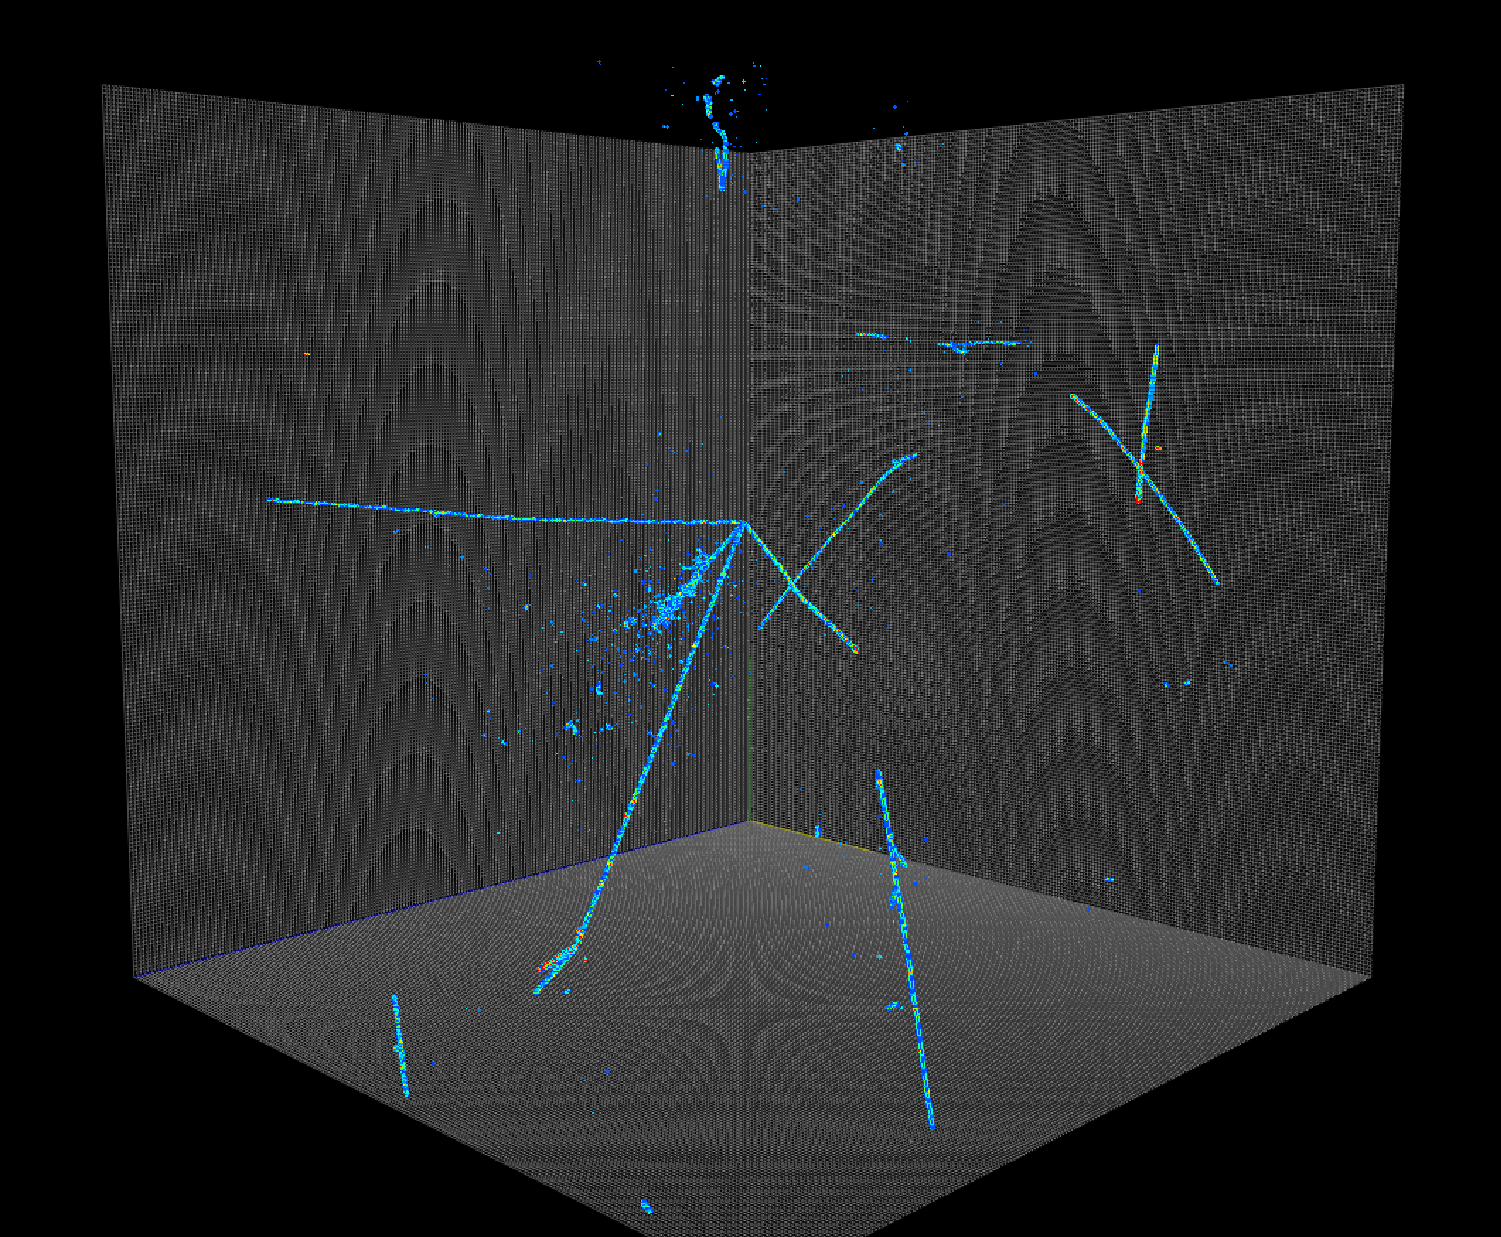
\includegraphics[width=0.48\textwidth]{figures/demo-data.pdf}
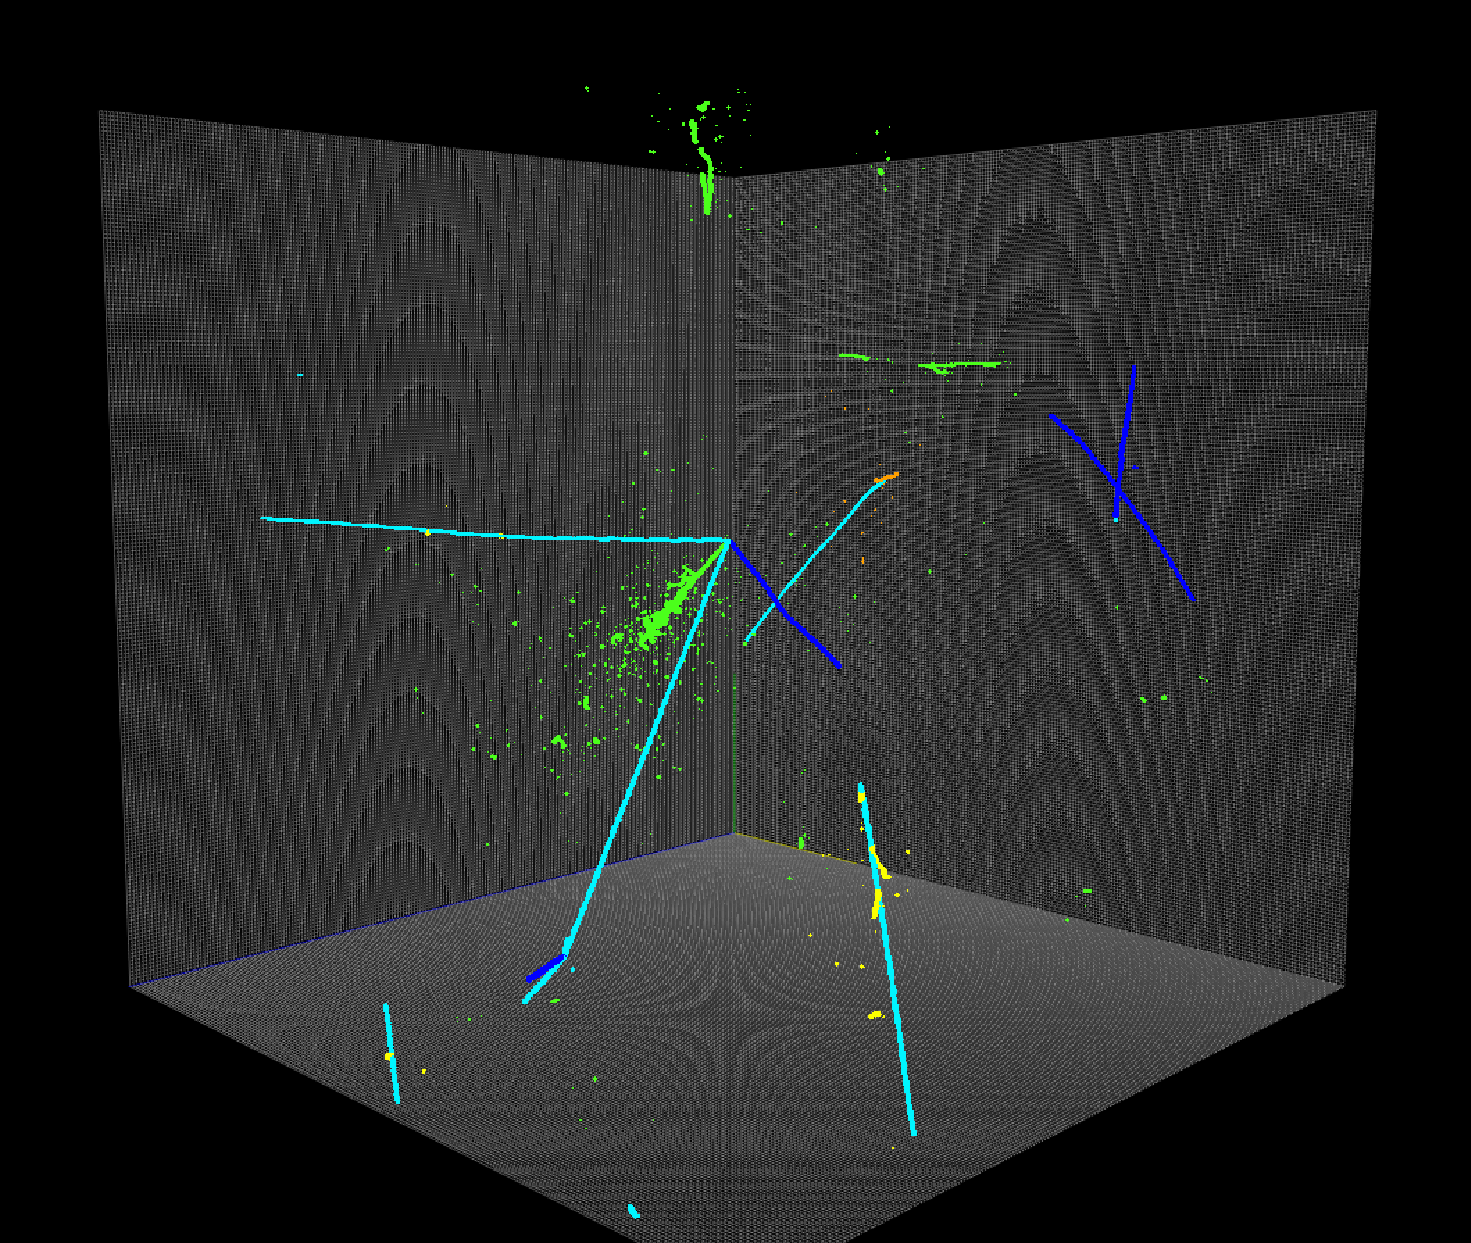
\includegraphics[width=0.47\textwidth]{figures/demo-label.pdf}
\caption{Example of a semantic segmentation task. The left shows the input image with particle trajectories where the continuous color scale corresponds to the amount of energy deposited by a particle in each pixel. The right shows different semantics (i.e. particle types) in a discrete set of colors.}
\label{fig:clustering:segmentation}
\end{figure*}
A semantic segmentation partitions data, image pixels, among the predefined set of categories (i.e. {\it semantics}). Two pioneering DNNs are the fully convolutional network (FCN)~\cite{long2014fully} and the U-Net~\cite{ronneberger2015unet}. Both of these belong to a family of convolutional neural networks (CNNs)~\cite{Fukushima1999,LeCun1999,NIPS2012_4824}, which have been extremely successful in the field of computer vision and established as the de-facto algorithm for image analysis. 

\subsection{Deep Neural Networks for Semantic Segmentation}
CNNs were first applied to and found to be successful~\cite{NIPS2012_4824,simonyan2014deep,szegedy2014going,he2015deep} for an image classification tasks, namely assigning an image to one of predefined set of categories (e.g. a cat vs. dog). A typical CNN for image classification consists of repeating blocks of convolution layers and pooling layers or strided convolution layers to downsample an input image in order to extract translationally invariant features at different spatial resolutions. This process gradually reduces the spatial size of an input data tensor and expands in the {\it feature} dimension, referred to as {\it channels} in image data. We refer to this as an {\it encoder architecture}, or simply an {\it encoder}, as what it does is to extract image features and encode into the feature dimension. At the end of an encoder is a block of fully-connected layers, which discards spatial information from the input data, to classify the whole image into one of several categories. Prior to this final block, a downsampled intermediate data tensor preserves information related to feature locations.
%Prior to this final block, although it is coarse due to previous down-sampling operations, an intermediate data tensor preserves the information about what features are present where. 

The FCN~\cite{long2014fully} explors the idea of reusing the spatial information in the output of a CNN encoder by replacing the last block of fully-connected layers with a $1\times1$ convolution layer. Intuitively this $1\times1$ convolution performs a semantic type classification at the downsampled, coarse pixel level. The goal of semantic segmentation is, however, to perform this classification at the spatial resolution of an input image. In order to do this, The FCN adds blocks of upsampling and convolutional layers. These blocks are essentially learnable interpolation algorithms. This process of transforming the encoded feature information back to a tensor of a high spatial resolution is referred to as a {\it decoding} architecture, or simply a {\it decoder}. The very last layer consists of $N+1$ filters where $N$ is the number of categories, or partitions, and one additional category represents the pixels that do not belong to any semantic type as background.

\begin{figure*}[t]
    \centering
    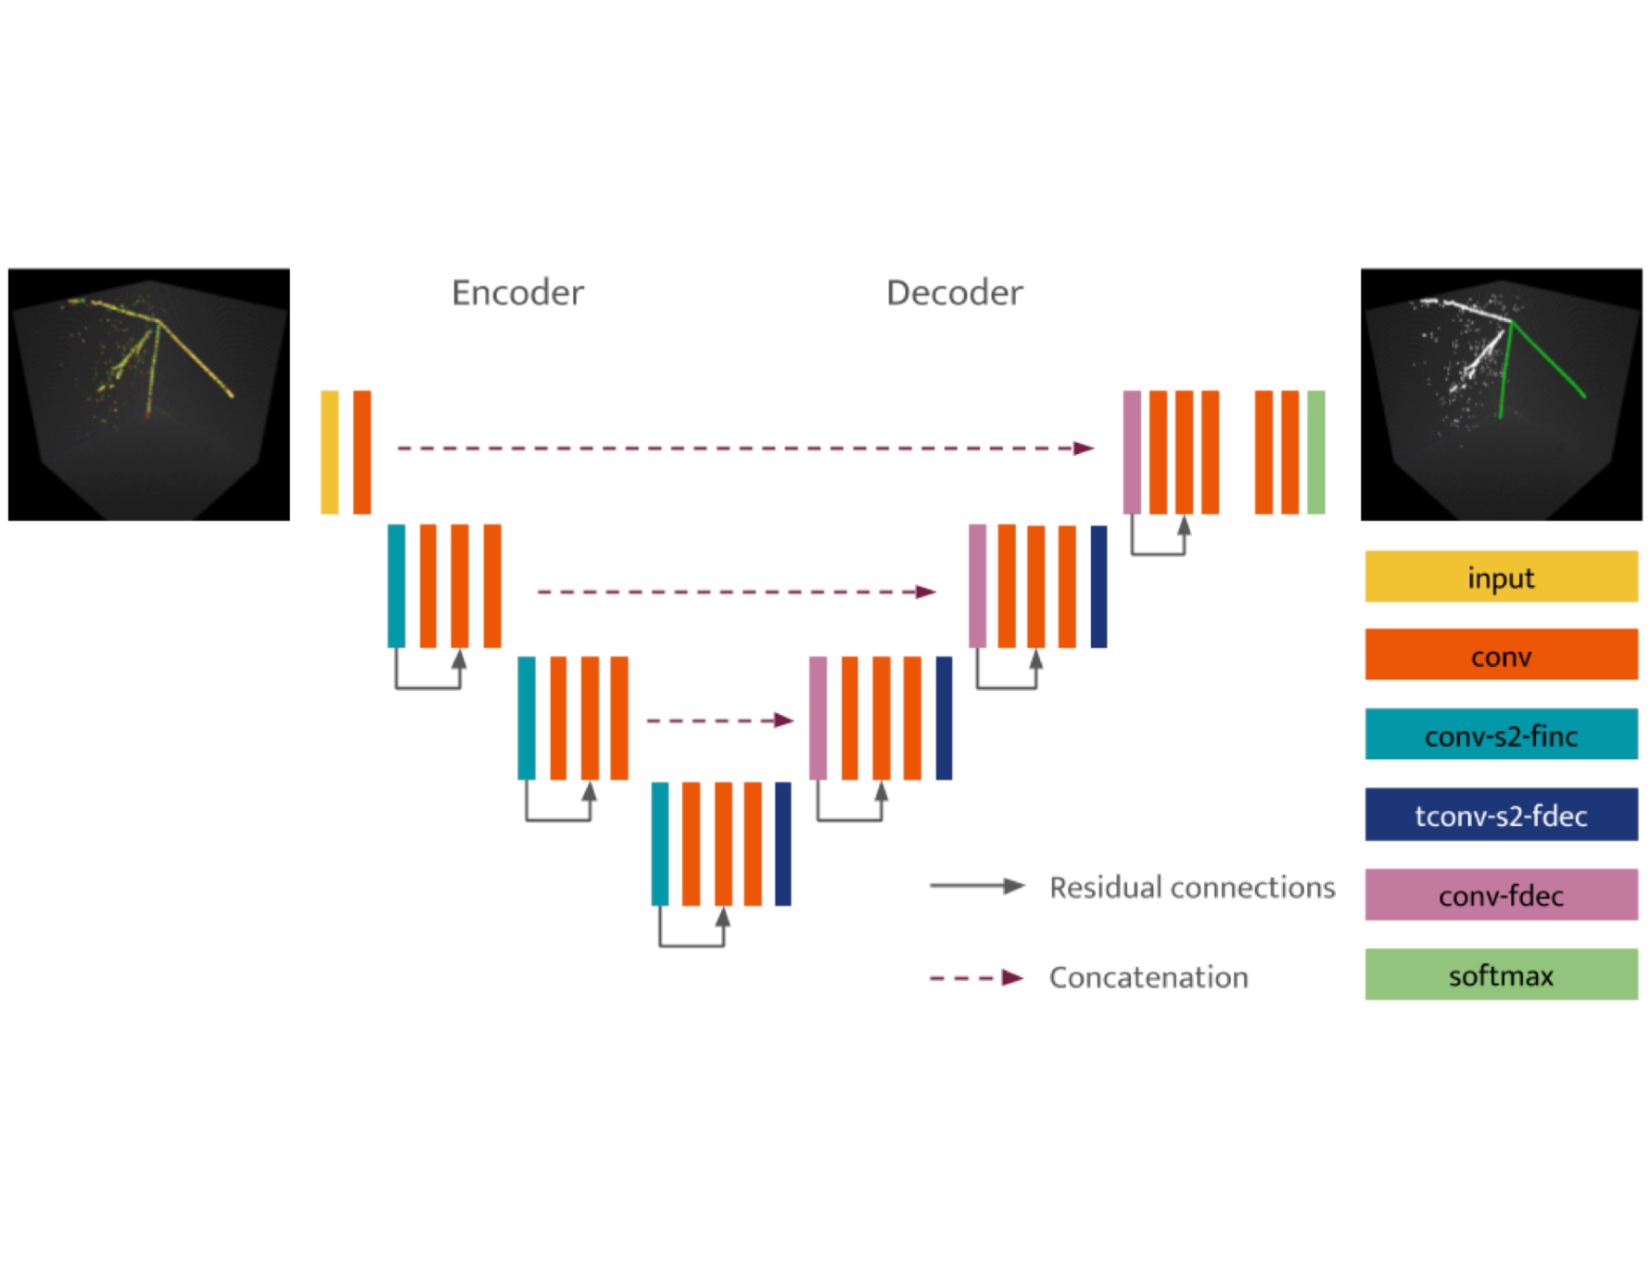
\includegraphics[width=0.98\textwidth]{figures/uresnet_architecture.pdf}
    \caption{Example implementation of a U-Net architecture for LArTPC neutrino detectors. The skip connections are shown in dashed arrows.}
    \label{fig:clustering:U-NetArchitecture}
\end{figure*}

The U-Net~\cite{ronneberger2015unet} extends the idea of the FCN, which, despite being a successful application of CNNs for semantic segmentation task, had limited spatial precision. The challenging aspect of FCN is that a full recovery of the spatial precision by an upsampling operation alone is impossible because the spatial information is evidently lost at the previous downsampling operations. In other words, the lost spatial information is present prior to each downsampling operation within the encoding blocks. U-Net exploited this fact by introducing {\it skip connections}, which is an operation to take a data tensor of corresponding size from the encoder and concatenate to the same, upsampled data tensor in the decoder.  An example architecture diagram is shown in Figure~\ref{fig:clustering:U-NetArchitecture}, taken from a U-Net implementation for a 3D imaging LArTPC detector~\cite{PhysRevD.102.012005}. With the skip connections, the lost spatial information is available to the convolution layers in the decoder, and results in a dramatic improvement in predicting the boundary of objects at the pixel level~\cite{ronneberger2015unet}.

\subsection{Semantic Segmentation in Neutrino Detectors}
\begin{figure*}[t]
    \centering
    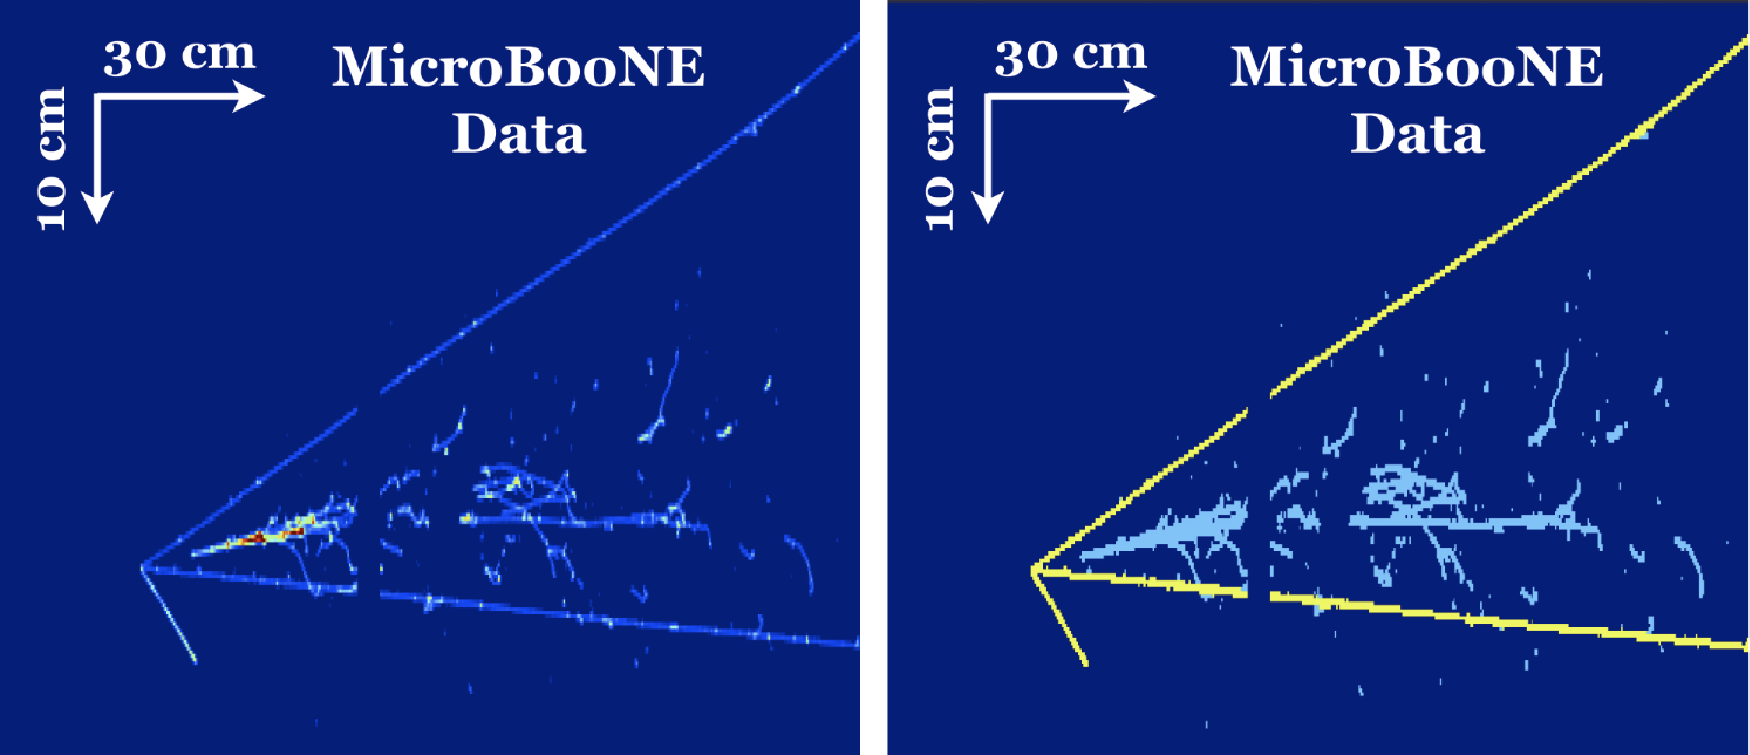
\includegraphics[width=0.98\textwidth]{figures/uresnet_uboone.pdf}
    \caption{Semantic segmentation applied in the MicroBooNE experiment to partition pixels into a track (yellow) and shower (cyan) categories.}
    \label{fig:clustering:UBooNE}
\end{figure*}
One of the first applications of semantic segmentation in particle physics was applied by the MicroBooNE experiment~\cite{PhysRevD.99.092001} using U-Net architecture with residual connections~\cite{he2015deep}, called U-ResNet, similar to the architecture shown in Figure~\ref{fig:clustering:U-NetArchitecture}. The goal of their application was to partition image pixels into two types: pixels that belong to a {\it track}, a trajectory with a line-like topology, and the others that belong to a {\it shower}, a trajectory with many branches and scatterings. Due to the distinct topological shapes, the two types of trajectories require very different algorithms in the next stage of data reconstruction chain where pixels are clustered into individual particle trajectories. Prior to U-ResNet, mixing of two topological types was a major bottleneck. Distinction of two types prior to this reconstruction stage was enabled for the first time using U-ResNet, and is now utilized for the downstream reconstruction chain in the experiment~\cite{collaboration2020vertexfinding}.  

U-ResNet in MicroBooNE is a supervised model that is trained using simulated image of particles. An assumption of this algorithm is that image features learned to perform the segmentation task are shared between data and simulation. A validation study is performed achieving percent-level statistical uncertainty~\cite{PhysRevD.99.092001}. As noted earlier, a study to confirm whether an implicit assumption of an algorithm holds or not is an important step for deploying a clustering algorithm. Beyond such a study, one may consider a strategy to actively mitigate discrepancies between the data and simulation domains. This challenge is called {\it domain adaptation} and is an active area of research in science including particle physics~\cite{wang2018deep,louppe2017learning,Perdue_2018}. 

\subsection{Scalable Sparse Segmentation for Big Data}
The scalability of an algorithm to bigger data is an important aspect of ML methods in particle physics. Despite its successful application, because of both its encoder and decoder blocks, U-Net requires more computation time and memory resources compared to widely used CNNs for image classification. The MicroBooNE study reported that they cropped a whole detector image that consists of more than 13 million pixels into a smaller frame, $512\times512$ pixels, in order to run U-ResNet. This means a factor of 50 reduction in size, and requires an extra processing stage to stick back the image to the original size before running the downstream reconstruction tasks. This is clearly not ideal. Moreover, the majority of pixels shown in example image data are backgrounds and do not contain information about a particle trajectory (e.g. see Figure~\ref{fig:clustering:UBooNE}), suggesting the majority of computation performed may be wasted. U-Net with standard convolutional layers is not scalable to bigger image data such as DUNE far detector (DUNE-FD), which will have a much larger volume, corresponding to 40 kiloton of LAr, 450~times more than that of the MicroBooNE detector.

Recently there have been two solutions proposed. The first is a class of sparse CNNs such as sparse submanifold convolutional networks~\cite{SSCN1,SSCN2} and Minkowski CNNs~\cite{choy20194d}. These frameworks provide implementation of fast linear algebra for sparse tensors while keeping the nature of CNNs, which is to extract translation invariant features from an image using small kernels. A successful application of U-ResNet with a sparse CNN framework has been pioneered for 2D and 3D LArTPC image data~\cite{PhysRevD.102.012005} where orders of magnitude improvement is reported in both wall-time and memory required for computation. It is worth noting that those computational resources required for sparse CNNs scale almost linearly with the number of {\it active pixels} in an image~\cite{PhysRevD.102.012005} (i.e. those pixels that carry values and are not {\it null}), and does not depend on the spatial size of the image. This makes segmentation algorithms like U-Net scalable to data from larger imaging detectors and also to higher dimensional data as it is already shown to work on 3D images.

\begin{figure*}[t]
    \centering
    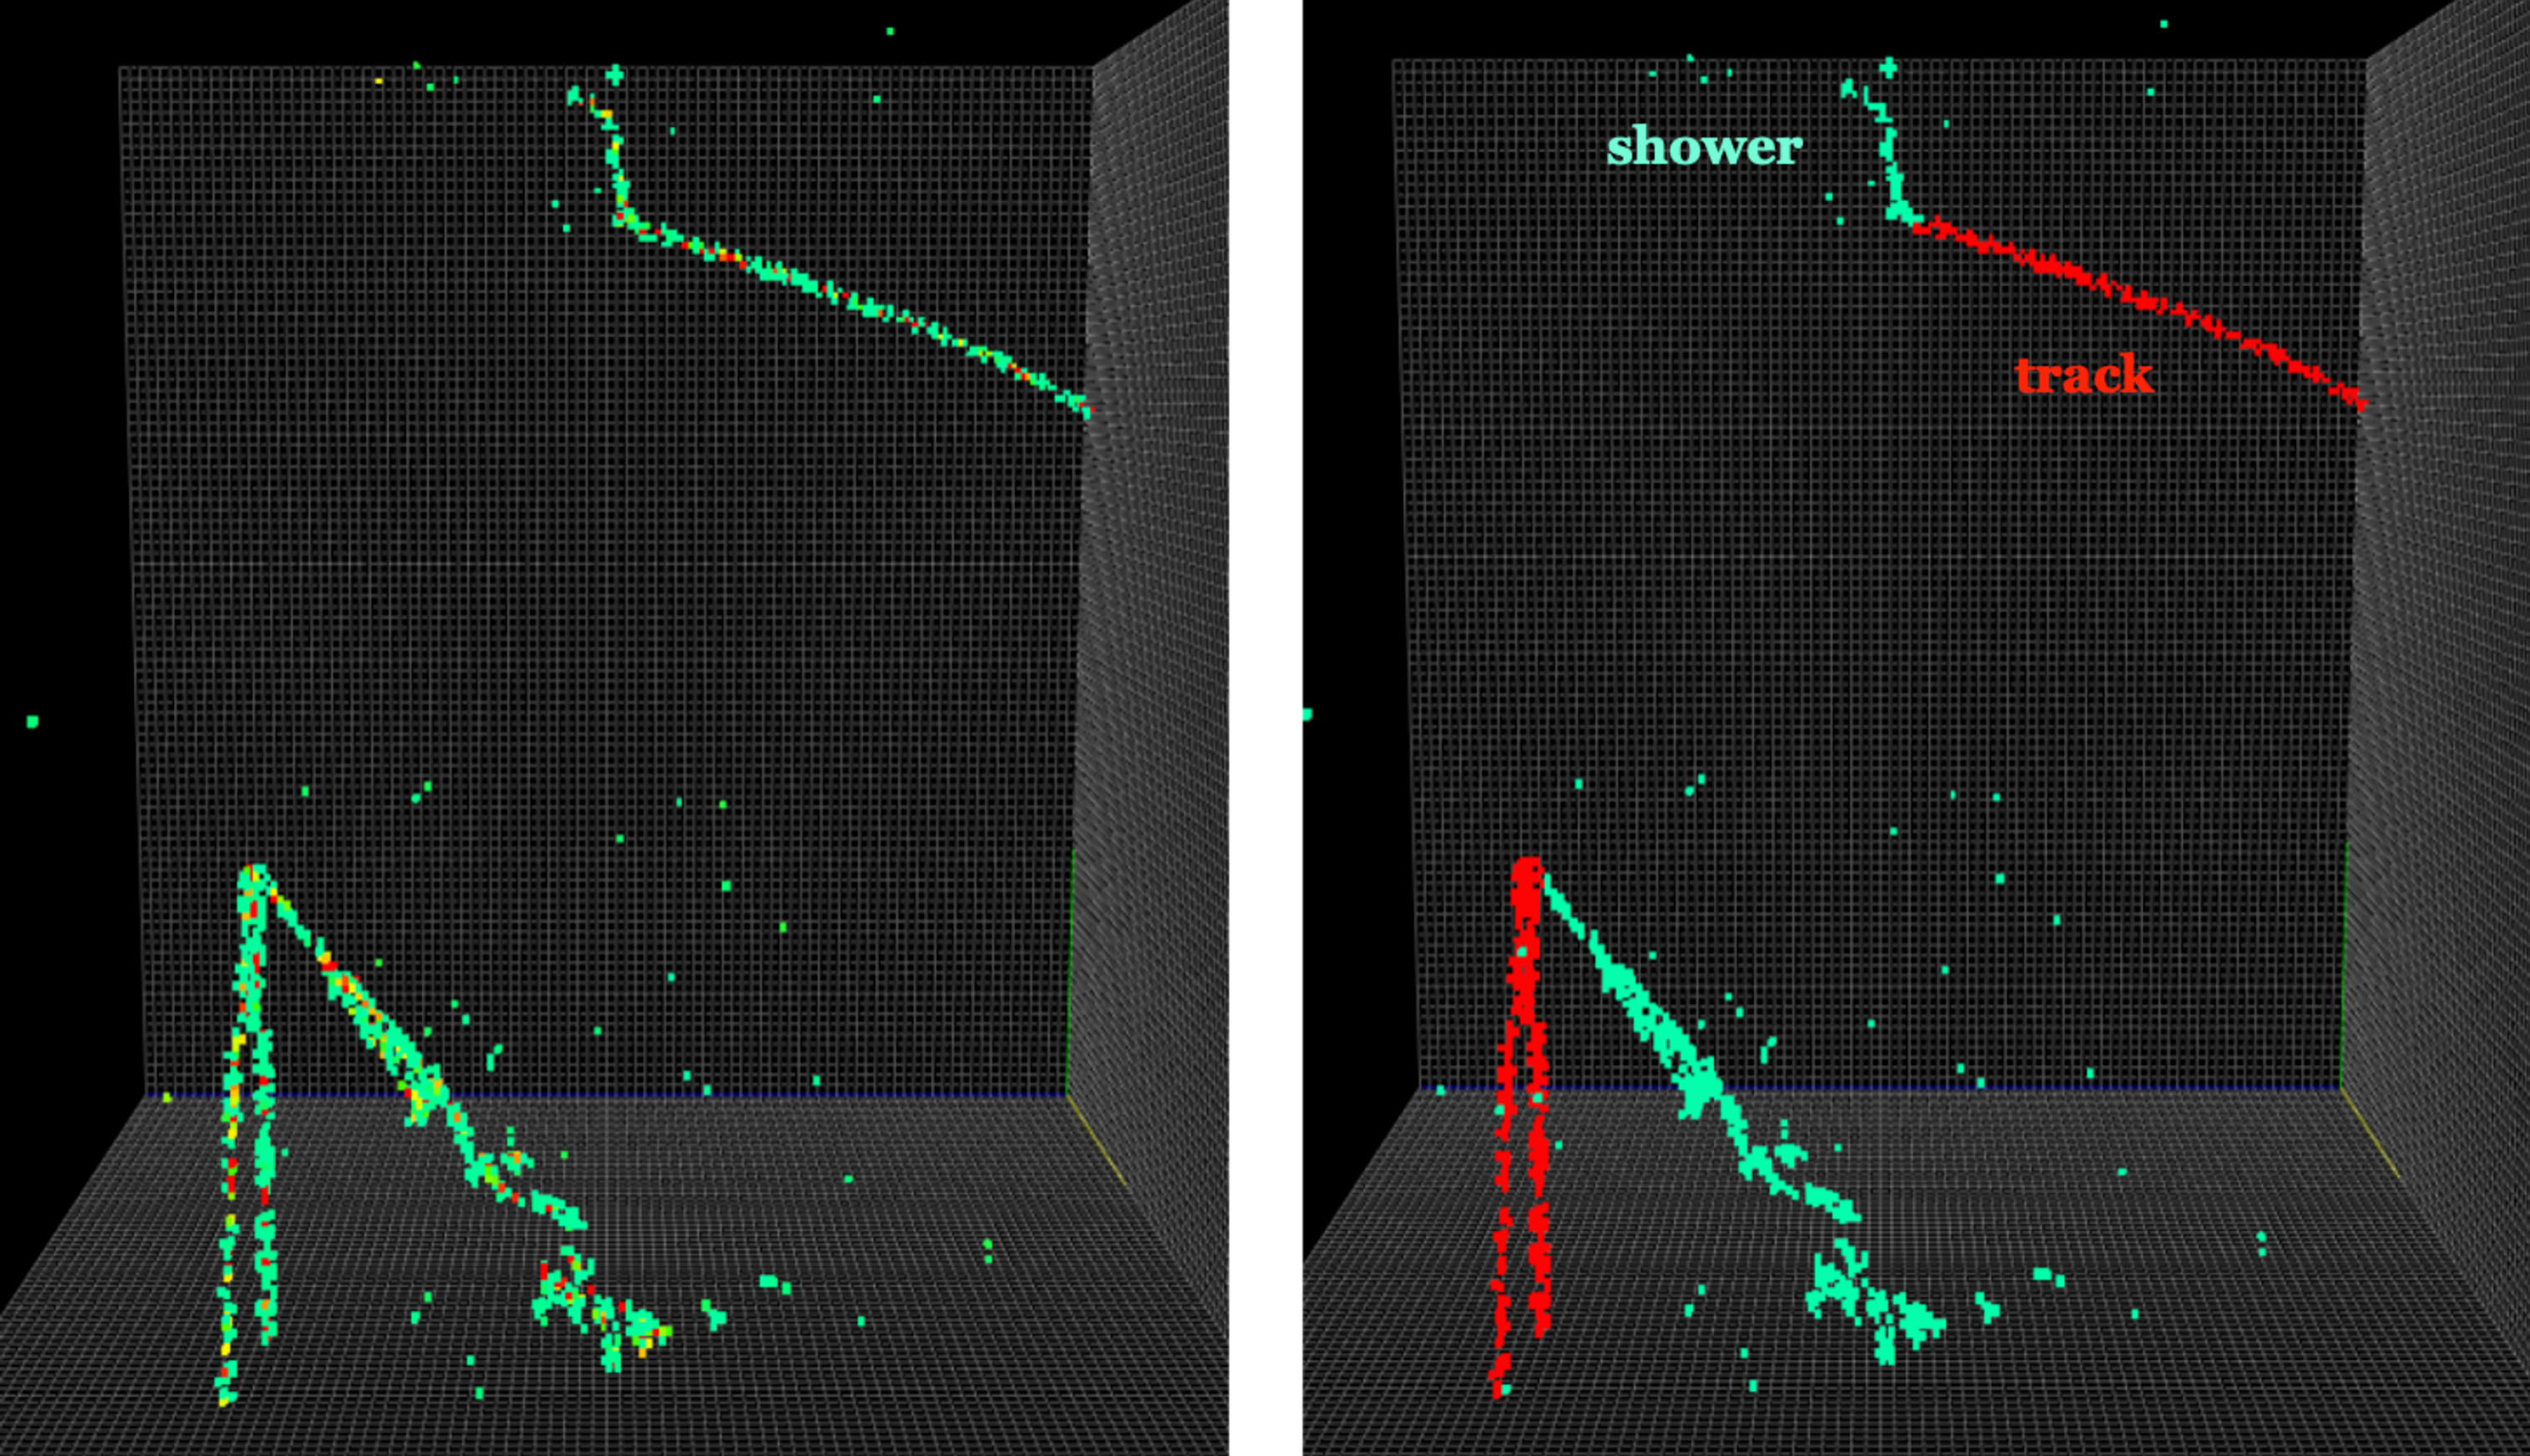
\includegraphics[width=0.98\textwidth]{figures/dgcnn.pdf}
    \caption{The dynamic graph CNN applied to simulated particle trajectory in a LArTPC detector. Particle trajectories with energy depositions in a continuous color scale is shown on the left. The network output is shown on the right with two distinct colors, green and red for shower and track pixels respectively.}
    \label{fig:clustering:dgcnn}
\end{figure*}
The second class of solutions consists of a graph neural network (GNN)~\cite{zhou2018graph}. In the case of semantic segmentation, an individual pixel could be interpreted as a graph {\it node}, and connected with neighboring nodes (i.e. neighboring pixels) through {\it edges}. This is analogous to a convolution operation in a CNN where a small kernel extracts translation invariant features.  Figure~\ref{fig:clustering:dgcnn} shows an output of a semantic segmentation task using the dynamic graph CNN (DGCNN)~\cite{Manessi_2020}, implemented by the author~\cite{drinkingkazu_dgcnn}.
%~\footnote{\url{https://github.com/DeepLearnPhysics/dynamic-gcnn}}
The performance for semantic segmentation is comparable to that of sparse CNNs in terms of both computational resource and task accuracy.

The choice between sparse CNN and GNN depends on the application, and it is important to note key differences. First, GNNs can be considered as generalization of CNNs in a sense that they do not require data points to be arranged in a fixed-size grid format (i.e. a matrix), and also there is flexibility to define arbitrary edges between nodes. The latter is important as it defines neighboring nodes to be involved in a convolution operation. On the contrary, CNNs act on matrix data and have much less flexibility in the convolutional kernels, which are typically a small rectangular matrix. It is also important to note that GNNs can effectively communicate information between nodes that are far apart in space by simply creating an edge between them. In contrast, in a CNN, an exchange of information between distant pixels is only possible after many downsampling operations, which also lacks fine spatial information as discussed earlier. While these facts appear advantageous to the use GNNs, the more flexibility means also the more phase space to be explored during training. In other words, if applied for appropriate tasks, limitations for CNNs can be considered constraints motivated by domain knowledge or inductive bias. If the input data is already in a matrix format, and if a proposed task does not require a large-scale feature that cannot be obtained by CNNs, the same or even better performance may be achieved using sparse CNNs. Few systematic comparison studies are performed, and none is published to the knowledge of the author at the time of this writing.

\subsection{Application to Michel Electron Clustering}
\begin{figure*}[t]
    \centering
    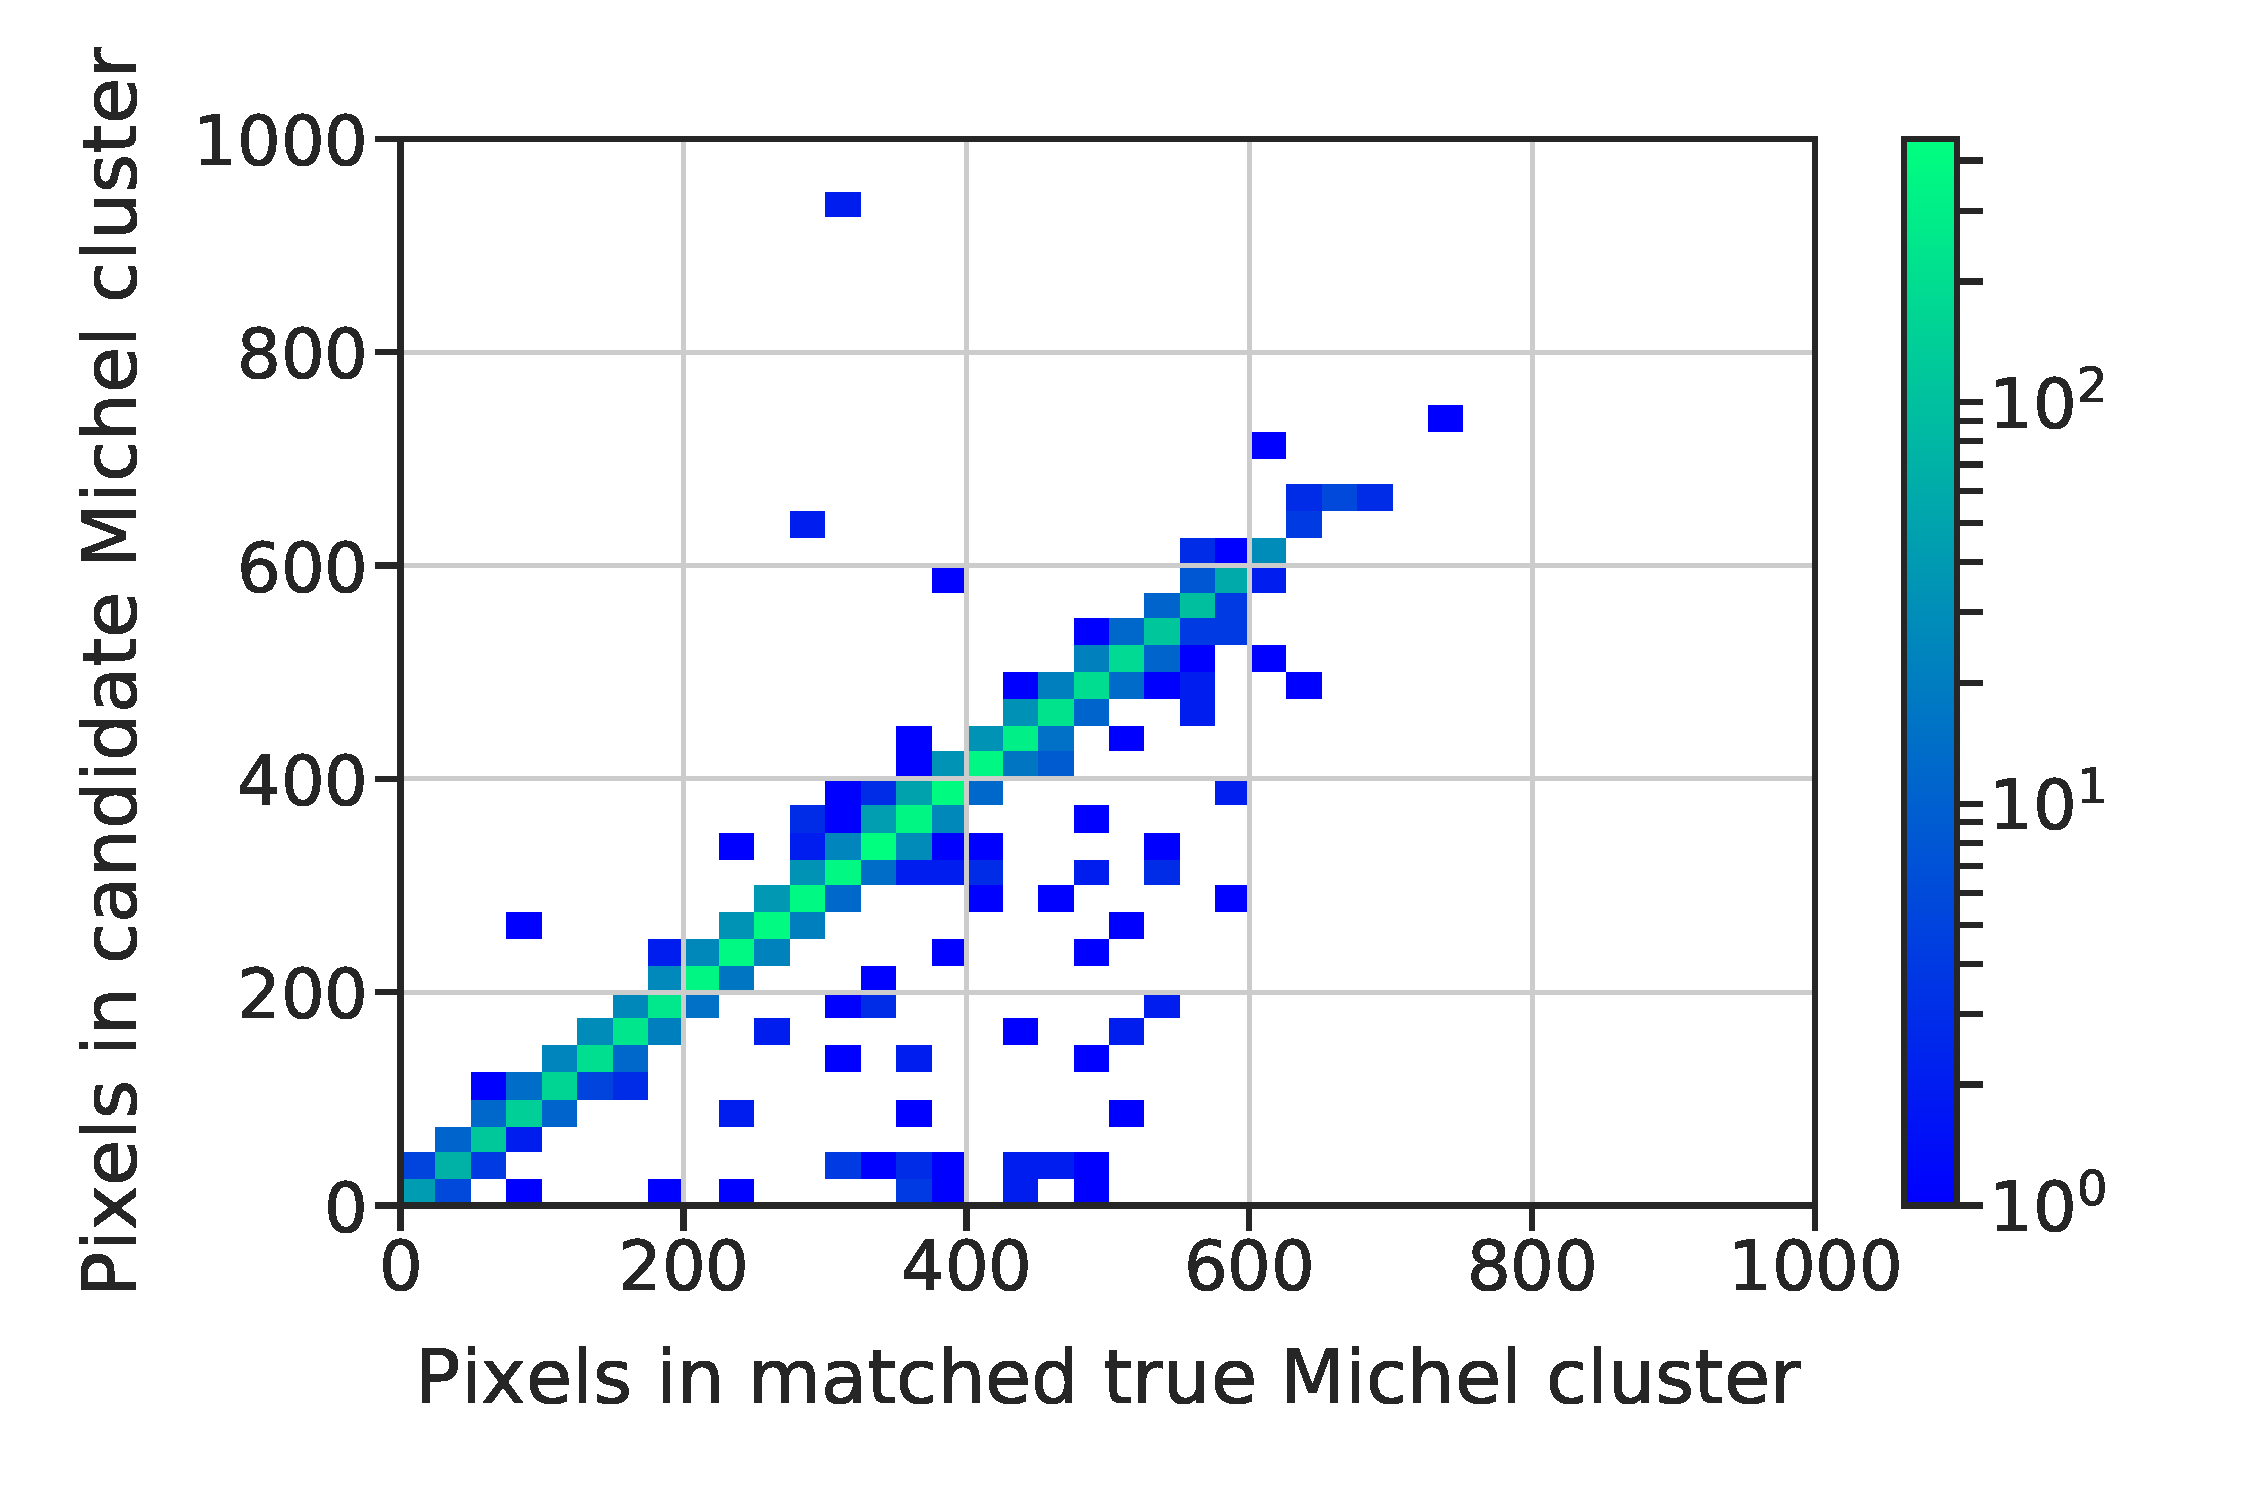
\includegraphics[width=0.75\textwidth]{figures/num_true_pix_vs_num_pred_pix3_new.pdf}
    \caption{Comparison of the pixel count between the true Michel electron clusters and the reconstructed ones. A reconstruction is matched to a true cluster based on the maximum overlap of pixels between them.}
    \label{fig:clustering:michel}
\end{figure*}
For some particles, running DBSCAN on a semantic segmentation mask is sufficient to cluster pixels and reconstruct a trajectory. A Michel electron from a muon decay in neutrino LArTPC detectors falls in this category as it is rare for two Michel electron trajectories to come in contact. As such, if a Michel electron is one of the semantic types, running DBSCAN on pixels labeled as Michel electrons by a semantic segmentation network would be sufficient to identify individual Michel electron trajectory. This is demonstrated by the authors of sparse U-ResNet paper~\cite{domine_laura_2018_1300713} using  3D particle simulation images in LAr where the Michel electron identification purity and efficiency are reported as 97~\% and 93~\% respectively. The pixel clustering purity and efficiency are both at 96~\%. Figure~\ref{fig:clustering:michel} from their paper shows a good agreement in pixel counts between reconstructed and true Michel electron clusters, where two class of clusters are matched using a criteria of maximum overlap in shared pixels.

\subsection{Application to Track Clustering}
\begin{figure*}[t]
    \centering
    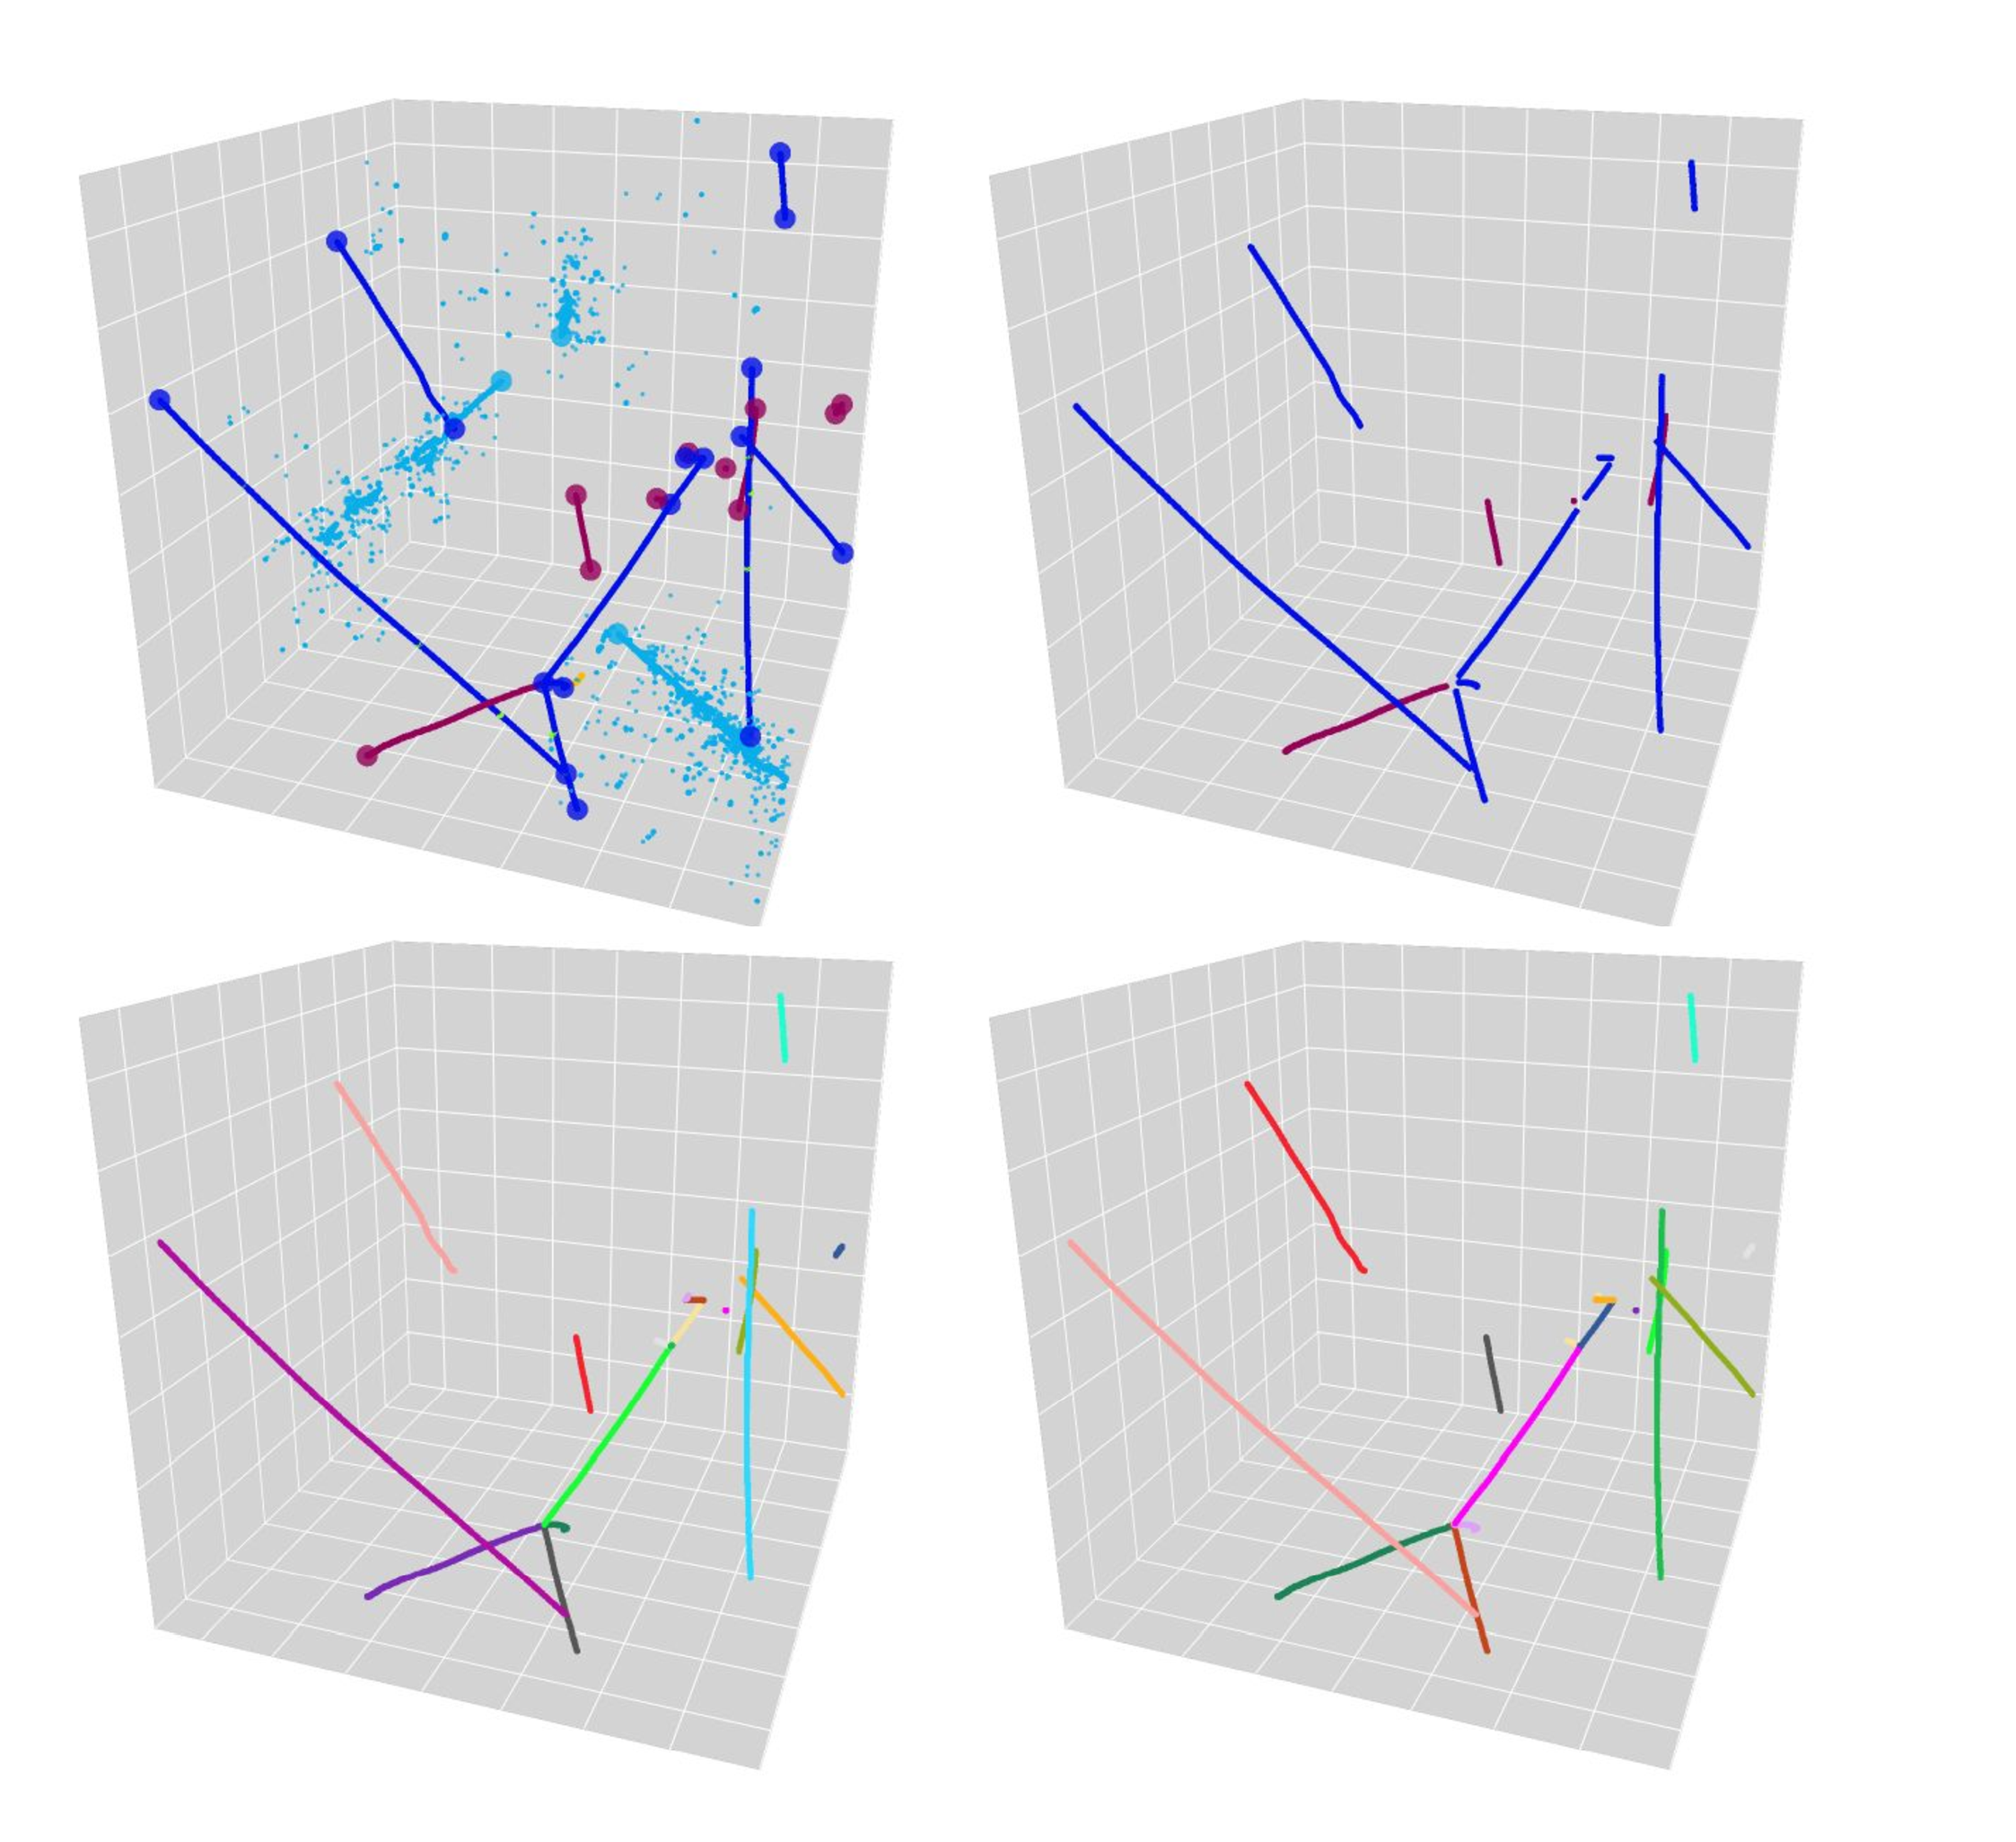
\includegraphics[width=0.98\textwidth]{figures/track_clustering.pdf}
    \caption{Application of semantic segmentation for a track clustering  using DBSCAN and PPN. The segmentation output with the endpoints of particle trajectories, found by PPN, are shown on the top-left. Then several pixels around those endpoints are masked out and DBSCAN is run for track pixels on the top right as an intermediate step. Distinct colors indicate distinct clusters in this and the bottom two images. Finally, the masked pixels are put back and assigned to the closest track cluster in the bottom right. The bottom left image shows the true underlying clusters. The coloring scheme is not meant to be identical between the bottom two images.}
    \label{fig:clustering:ppn_track_clustering}
\end{figure*}
Clustering of pixels into track particle trajectories seem to be a simple task after those pixels are separated from shower particles that exhibit more complicated shapes. Since the trajectory of a track particle is simply a continuous line, DBSCAN seems to be a reasonable choice of an algorithm to cluster its pixels. When two track particles originate from the same point (e.g. at an interaction vertex, or a decay point), it may need to be broken at the connection point. This is implemented in the work of Point Proposal Network (PPN)~\cite{Domine:2020tlx,domine_laura_2018_1300713}, which consists of a few sparse convolution layers that work in conjunction with U-ResNet. The objective of PPN is  detection of endpoints of particle trajectories and position regression of those points. Using the Region CNN (R-CNN) architecture, which has been known to be the most successful architecture for detecting objects in an image, PPN can detect an arbitrary number of trajectory endpoints accurately. A proposed clustering algorithm is extremely simple. First, U-ResNet and PPN are run so that pixels are classified into track semantic types and endpoints are detected. Secondly, all pixels that are within 7 pixels from all endpoints are masked out, and DBSCAN is run to cluster individual track particle trajectory. Thirdly, masked pixels are put back, and assigned to the closest track cluster near the masking boundary. Figure~\ref{fig:clustering:ppn_track_clustering} is taken from the PPN work~\cite{Domine:2020tlx} and visualizes these steps. This is a simple extension to an algorithm with a fixed partitions, like U-ResNet, to allow clustering of arbitrary number of particle trajectories.

A short-coming of DBSCAN, namely an assumption of a single-valued point density, however, remains as a concern in such a clustering algorithm. From the nature of LArTPC, the thickness of a particle trajectory is known to depend on multiple factors including the diffusion of ionization electrons during drift and the angle of a trajectory with respect to the charge readout plane, to name a few. Moreover, at the interaction vertex, where multiple particles may come out and is of the most interest for neutrino physics analysis, the density ultimately depends on the multiplicity and type of particles produced. When considering these factors, the point density near the particle endpoints is definitely not single-valued, and is more likely continuous. Aside from track particles, DBSCAN would not be a solution for shower particles whose trajectory consists of many fragments with gaps of wildly varying sizes in between due to 15--30~cm radiation length in LAr. ML algorithms that are capable to {\it learn} complex underlying image features are needed to address the challenge of pixel clustering in these LArTPC image data, and they are discussed in the following text.

\section{Convolutional Neural Network for Pixel Clustering}
\begin{figure*}[t]
    \centering
    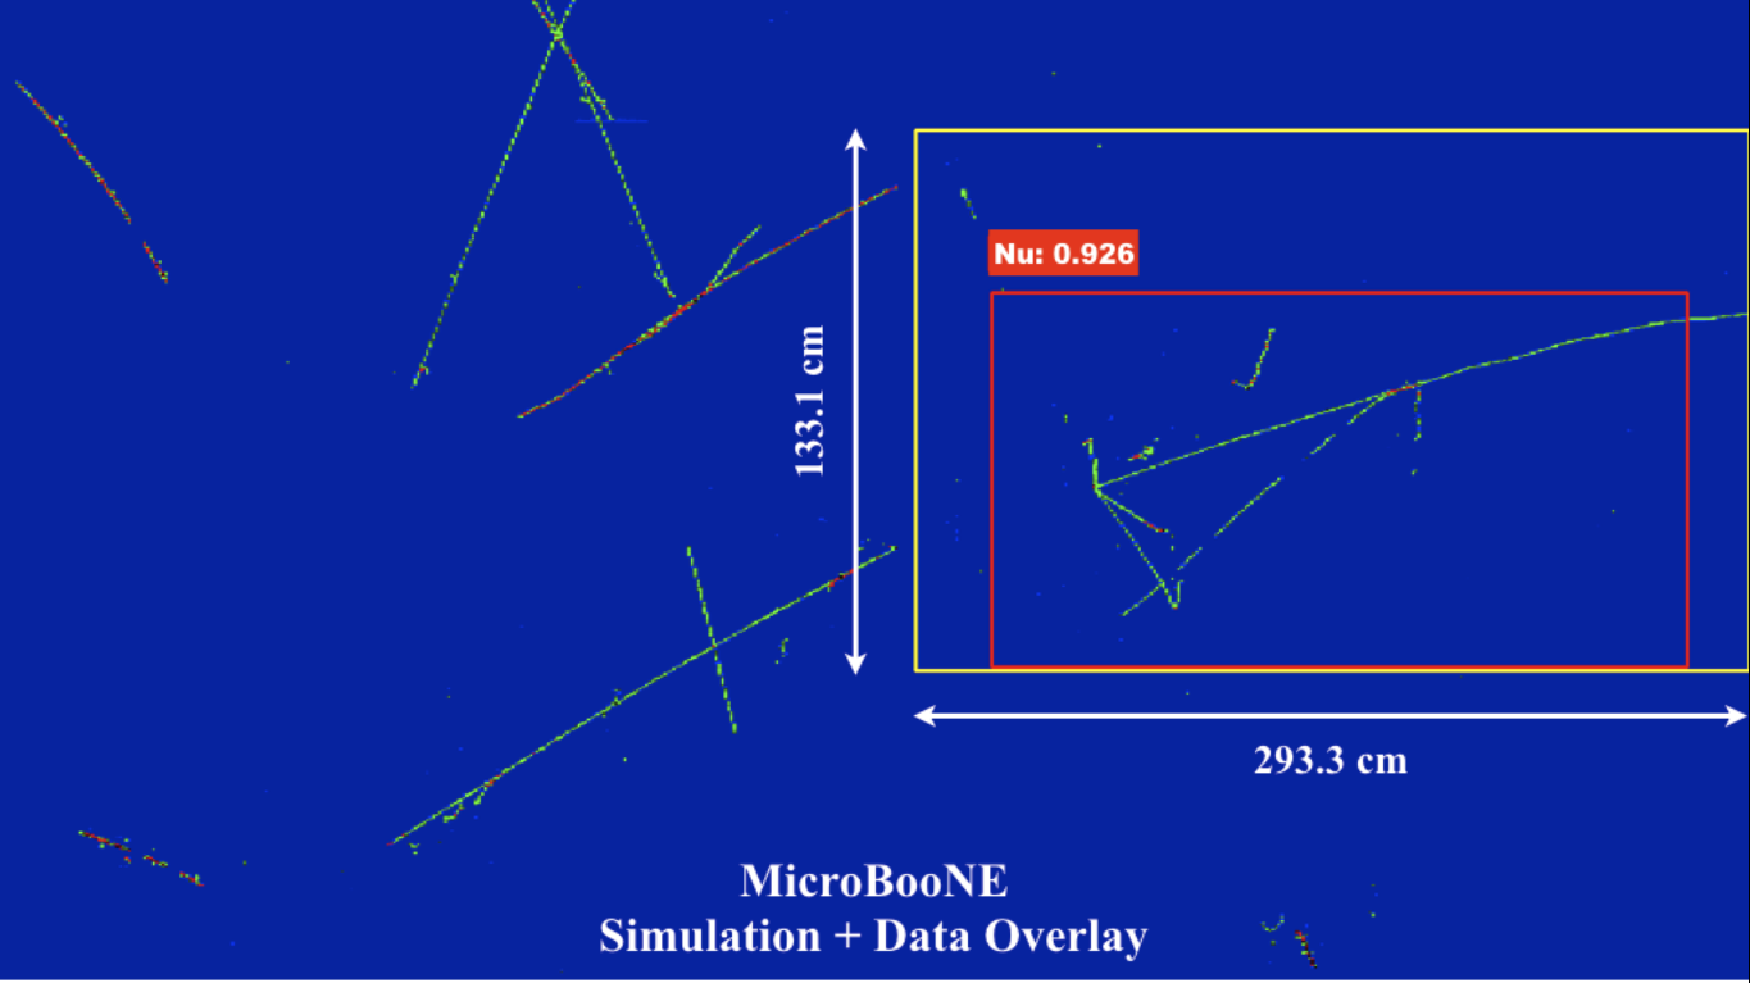
\includegraphics[width=0.98\textwidth]{figures/uboone_detection.pdf}
    \caption{Faster R-CNN object detection network applied in MicroBooNE experiment. The location and the size of a boundary box shown in red are produced by the algorithm while the true refrence is shown by the yellow boundary box. }
    \label{fig:clustering:uboone_detection}
\end{figure*}
Clustering of image pixels in order to identify an individual instance of an object in an image is a task called {\it instance segmentation} and has been an active area of research in the field of computer vision.  There are two well known approaches to this task. The first is based on an object detector, such as R-CNN. 
This class of a solution works in two steps: the first step detect individual object location and size in the form of a bounding box (see Figure~\ref{fig:clustering:uboone_detection} for example), then the second step identifies pixels that belong to the target object within the bounding box. This class of a solution is referred to as {\it proposal-based approach} in the following text. The second class of a solution is to use CNN to learn a function which can transform image pixels into an embedding space where the clustering task may be much simplified. For instance, a loss for a CNN may be conditioned with objectives similar to $k$-means by enforcing pixels that belong to the same particle trajectory to gather close to each other in embedding space, ultimately to the same embedding coordinate. If successful, a simple algorithm such as DBSCAN may be employed in the embedding space to cluster pixels more easily.

%This class of a solution first gathers proposals of a {region of interest} (ROI), typically a rectangular bounding-box that contains an object instance in the image, by running an object detector. Figure~\ref{fig:clustering:uboone_detection} shows an example from the MicroBooNE experiment~\cite{Acciarri_2017,Radovic2018} where Faster R-CNN~\cite{renNIPS15fasterrcnn}, an object detection algorithm, is applied to locate a neutrino interaction in an image. In the next step, pixels within the bounding box that belong to the target object are identified. This class of a solution is referred to as {\it proposal-based approach} in the following text. 

%The second class of a solution is to use CNN to learn a function which can transform image pixels into an embedding space where the clustering task may be much simplified. For instance, a loss for a CNN may be conditioned with objectives similar to $k$-means by enforcing pixels that belong to the same particle trajectory to gather close to each other in embedding space, ultimately to the same embedding coordinate. Further constraints may also be useful, such as keeping large distances between the centroid of clusters among different particle trajectories. If successful, a simple algorithm such as DBSCAN may be employed in the embedding space to cluster pixels more easily.


\subsection{Region-Proposal Approach}
\begin{figure*}[t]
    \centering
    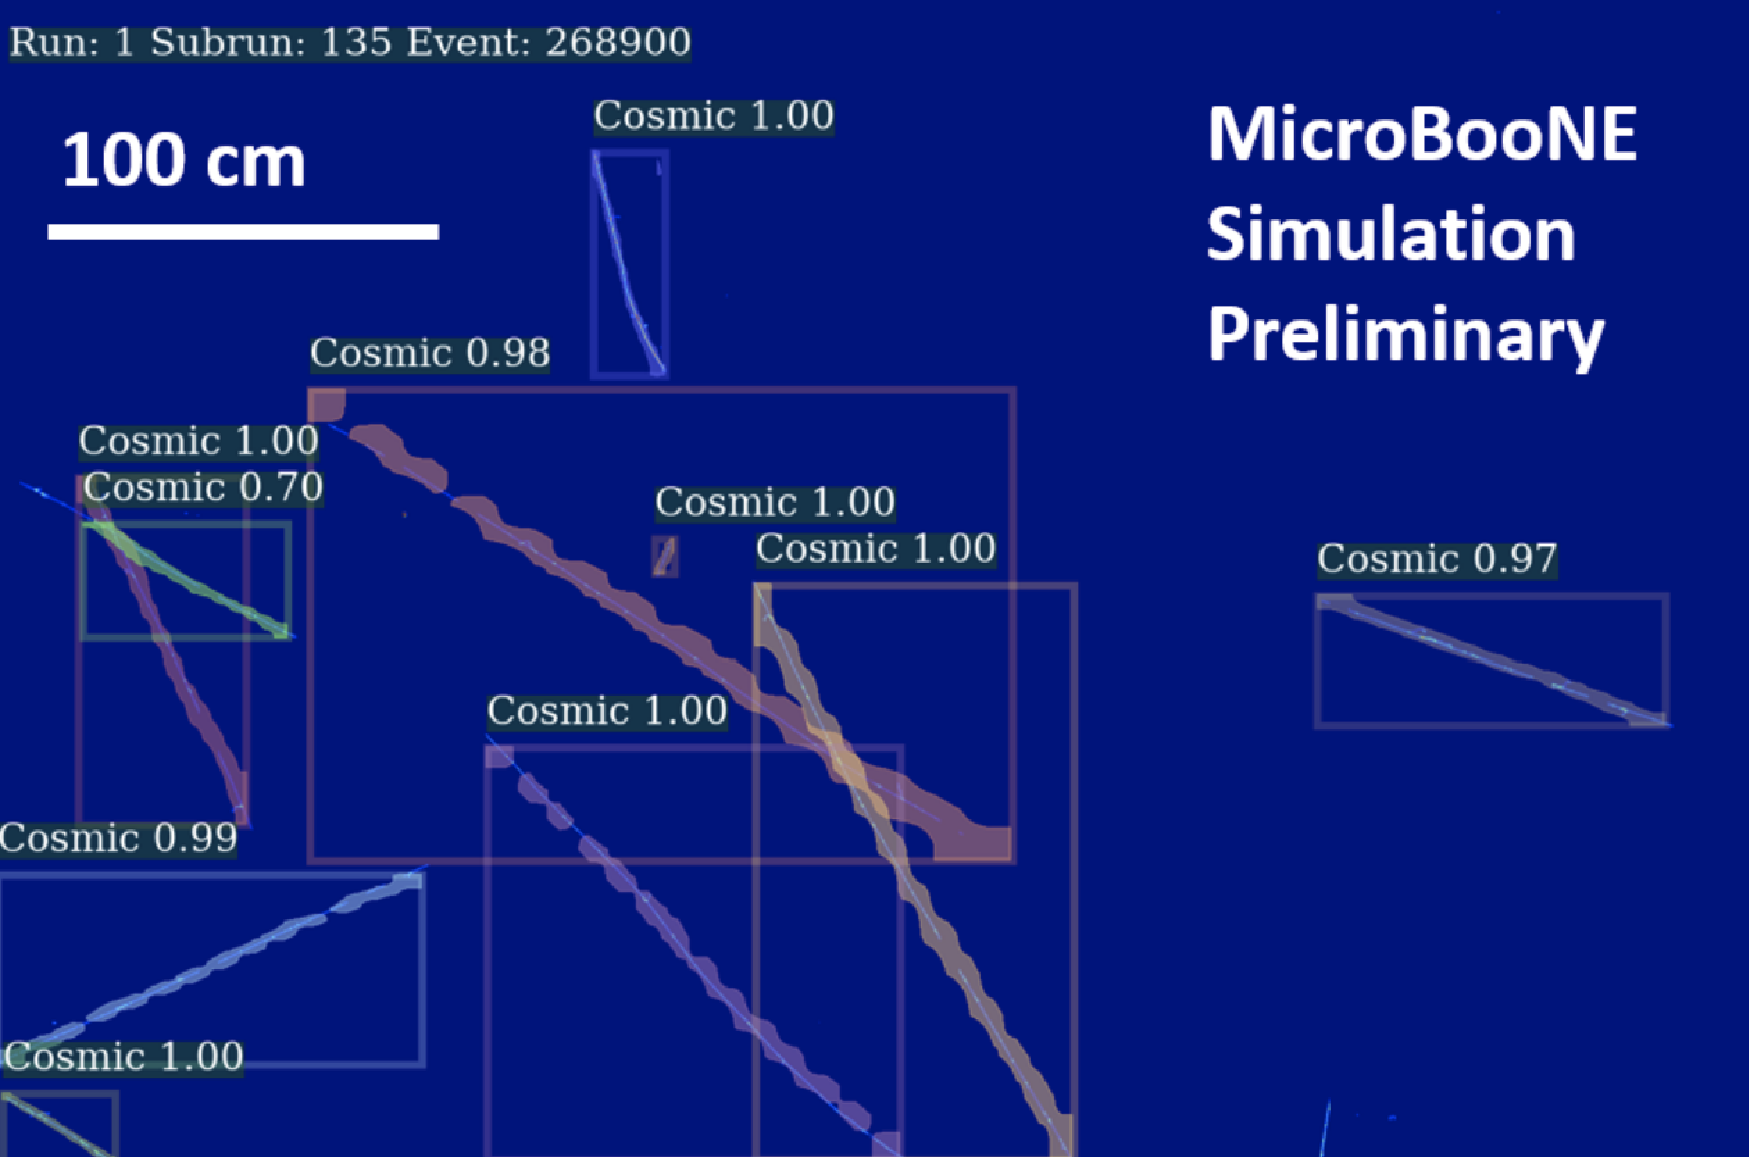
\includegraphics[width=0.9\textwidth]{figures/uboone_maskrcnn.pdf}
    \caption{Mask R-CNN applied in MicroBooNE experiment to identify individual cosmic ray trajectories. A rectangular box indicates an identified particle. Partially transparent masks are generated by a masking network.}
    \label{fig:clustering:uboone_maskrcnn}
\end{figure*}
{\bf MRC: This paragraph seems redundant with the first paragraph of section 3. I would take some of the detail out of that pararaph, and make it coherent with this one.}
One popular approach to instance segmentation is a CNN that employs a region-proposal method such as R-CNN. CNNs of this type consists of three components. The first is an encoder architecture for extracting image features. The second is a region proposal network (RPN) which detects arbitrary number of object locations and propose a bounding box, or ROI, per instance. The third is a semantic segmentation network, such as Fully Convolutional Network (FCN)~\cite{long2014fully}, which generates an instance {\it mask} by classifying all pixels within each ROI into the foreground (i.e. instance) or the background. One of the most successful algorithms in this class is called Mask R-CNN~\cite{8237584} which uses a Faster R-CNN for an object detection with a FCN for an instance masking.  Mask R-CNN is widely used in computer vision and neutrino experiments including NOvA and MicroBooNE for identifying particle instances in an image.  Figure~\ref{fig:clustering:uboone_maskrcnn} shows an implementation in MicroBooNE experiment for identifying individual cosmic-ray trajectories, important backgrounds to be removed in their neutrino analysis.

Despite the success of Mask R-CNN in many applications, however, the approach using region-proposal mechanism is prone to a few challenges. First, as this technique reduces the segmentation challenge within the proposed region of interest, a misplaced bounding box has a direct consequence in loss of clustering performance. If pixels that are part of the target object are  not within its bounding box, they are simply lost. Second is an {\it object occlusion} issue: two instances of the same type and bounding boxes of a similar position and size become inherently indistinguishable. Furthermore, as a domain-specific challenge, a rectangular bounding box is far from ideal to represent the region of a particle trajectories and results in a large number of background pixels. It currently remains as an active area of research to overcome these challenges and implement Mask R-CNN and other family of region-proposal algorithms for clustering pixels in data reconstruction.

\subsection{Proposal-Free Approach} 
\begin{figure*}[t]
    \centering
    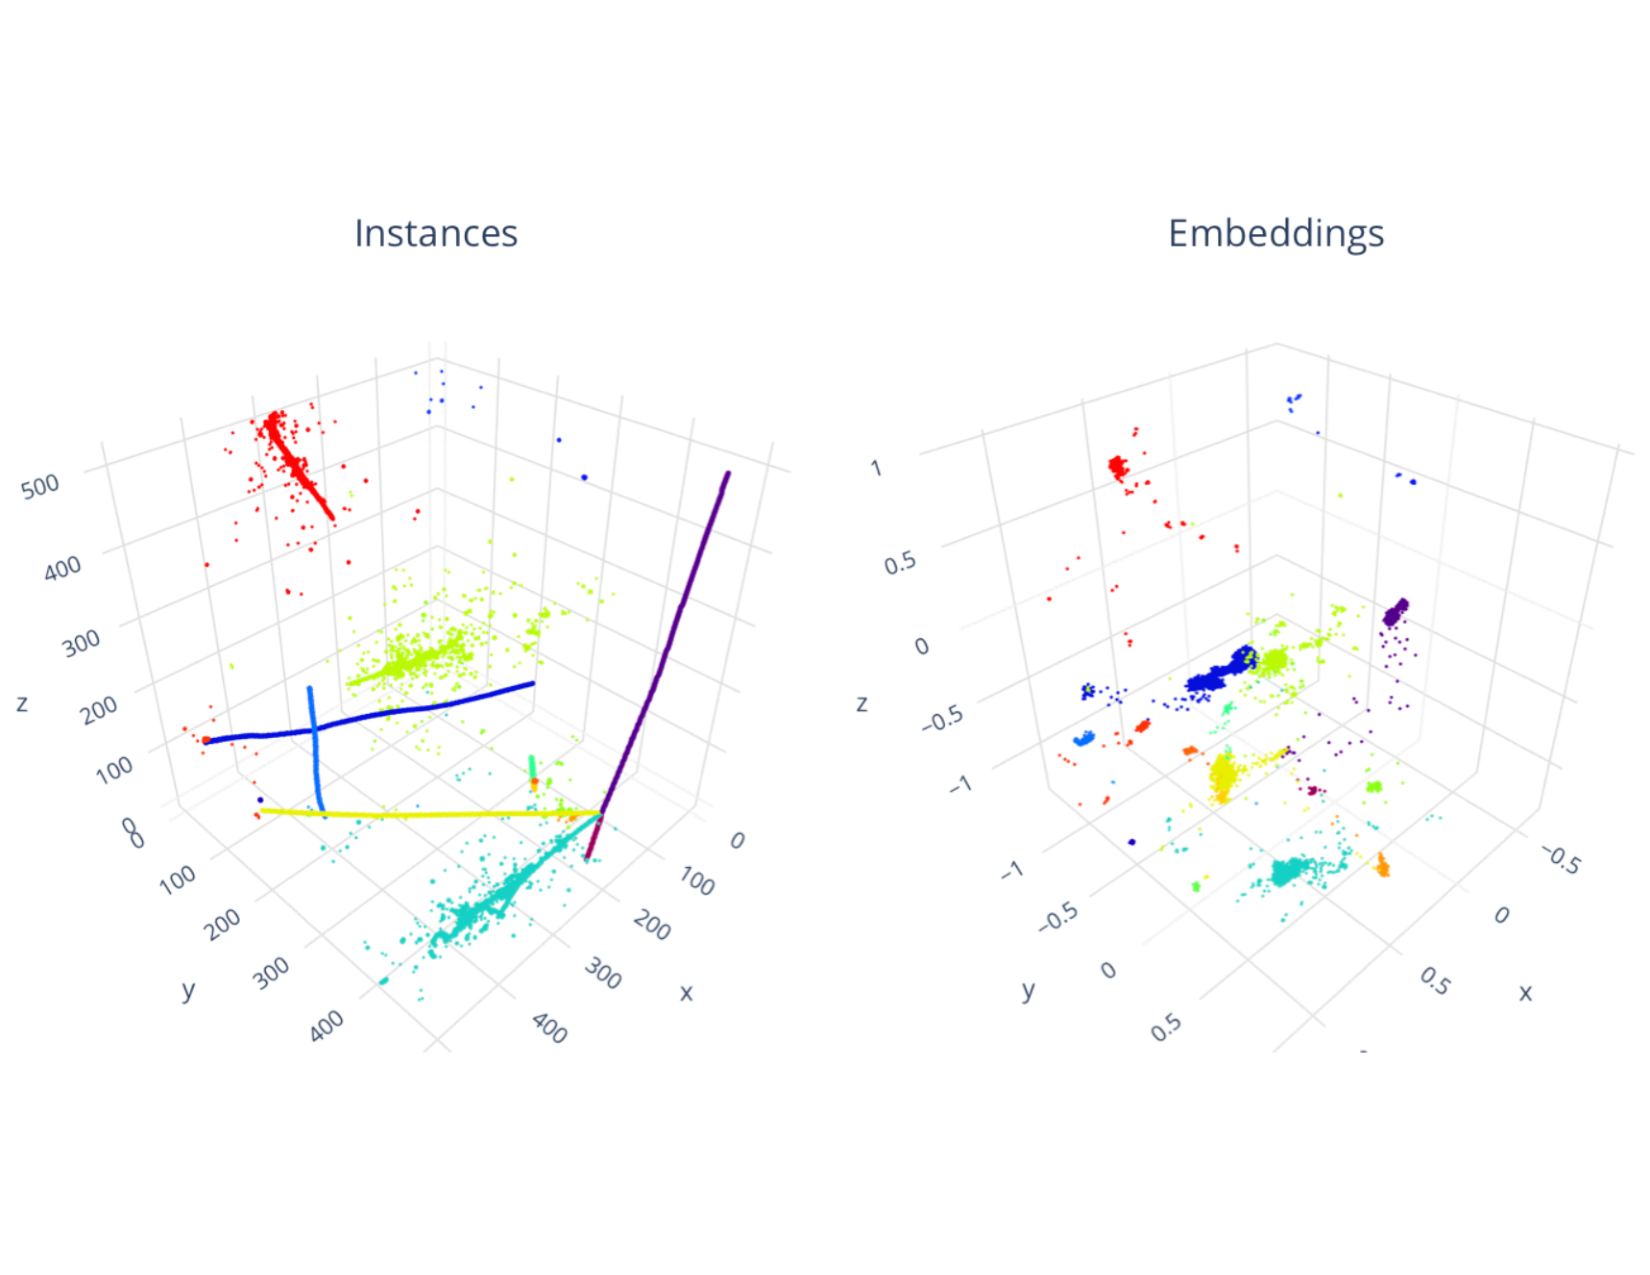
\includegraphics[width=0.98\textwidth,trim=0cm 3cm 0cm 3cm, clip]{figures/prediction_24.pdf}
    \caption{Transformation of pixels from the 3D image space (left) into the 3D embedding space (right) by SPICE. Pixel colors are discrete, and those ixels that belong to the same particle trajectory (cluster) shares the same color. }
    \label{fig:clustering:spice_embedding}
\end{figure*}
Proposal-Free approaches avoid reducing the segmentation challenge only within proposed ROIs. One of the most successful solutions in this class is a pixel coordinate transformation, which is to transform pixel coordinates from the original image space to $n$-dimensional embedding space. Scalable, Proposal-free Instance Clustering in Embedding (SPICE) is introduced for analyzing 3D LArTPC image data. It is based on sparse CNN with an architecture similar to U-ResNet, and is specifically for clustering densely connected pixels for which CNNs are well suited. SPICE transforms pixels from the 3D image space, $I\in\mathbb{Z}^3\times\mathbb{R}$, represented by three integer coordinate values and one floating point pixel value, into the 3D embedding space $\mathbb{R}^3$. Figure~\ref{fig:clustering:spice_embedding} shows the coordinates of pixels in both the image and embedding space~\cite{koh2020scalable}.

\begin{figure*}[t]
    \centering
    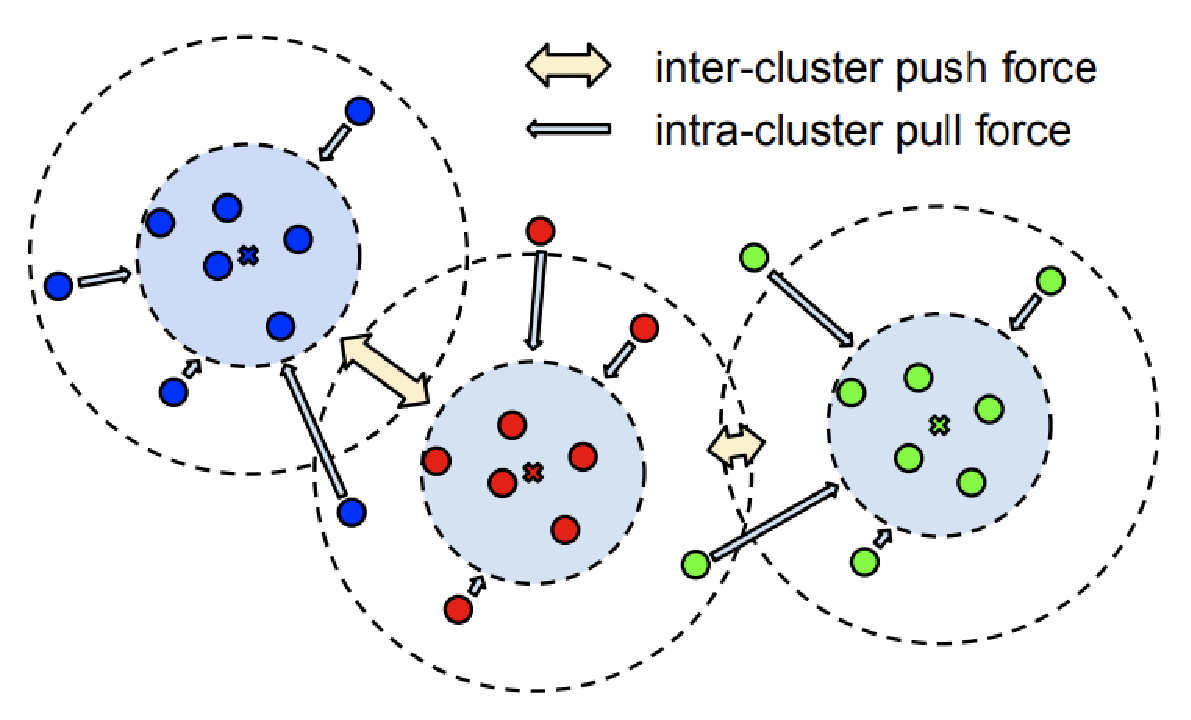
\includegraphics[width=0.65\textwidth]{figures/embedding_loss.pdf}
    \caption{$\mathcal{L}_{var}$ and $\mathcal{L}_{int}$ act as a force to pull pixels to the cluster centroid and to repel centroids of different clusters respectively.}
    \label{fig:clustering:embedding_loss}
\end{figure*}

\subsubsection{Embedding Loss}
The original work~\cite{disc}, from which SPICE is derived, employed the embedding loss, $\mathcal{L}_{emb}=\mathcal{L}_{var}+\mathcal{L}_{int}+\mathcal{L}_{reg}$, in order to condition the transformation process. $\mathcal{L}_{var}$ represents the variance of pixel coordinates with respect to the centroid of a cluster to which they belong. $\mathcal{L}_{int}$ concerns the distance between the centroids of clusters, and rewards the algorithm for keeping a certain inter-cluster distance. Finally, $\mathcal{L}_{reg}$ is a linear sum of distance to the centroid from the origin of the embedding space, which acts as a L1 regularization loss to place clusters near the origin. The effect of $\mathcal{L}_{var}$ and $\mathcal{L}_{int}$ are visualized in Figure~\ref{fig:clustering:embedding_loss} from the original work~\cite{disc}. These essentially work as pulling force to gather pixels to the centroid of their clusters and repelling force between the centroids of different clusters. 

While these are intuitive conditions for defining the transformation, there still needs to be a step to actually cluster pixels in embedding space. In the original work, Mean-Shift~\cite{1000236} was employed, which is not a learnable algorithm. The short-coming in this approach is that the actual clustering step in the post-processing is not a part of the algorithm optimization, and hence the embedding space may become sub-optimal. 

\subsubsection{Joint Optimization of Embedding and Clustering}
More recent work~\cite{8953222} incorporates the pixel clustering step and its loss so that the whole pipeline of pixel clustering can be optimized end-to-end. In this  work, in addition to the coordinates in embedding space, two additional parameters are estimated by the algorithm for every pixel: a cluster {\it margin} and {\it seediness} of a pixel. The seediness is a measure of how likely a pixel may represent the centroid of a cluster to which it belongs in embedding space. The margin is the spread of pixels with respect to the centroid of the cluster to which a pixel may belong. The margin loss is conditioned to minimize the spread of margin values across pixels that belong to the same cluster. However, a margin value is allowed to vary among clusters to accommodate the fact that there are variations in the size and confidence of the cluster (i.e.  ``difficult'' clusters may have a larger margin). Finally, the embedding loss is conditioned such that the pixels follow a normalized gaussian distribution around the centroid of a cluster. In the inference, pixels are ordered from high to low seediness score value. Given a candidate seed pixel, a score that indicates whether or not another pixel belongs to a candidate cluster represented by this seed pixel can be calculated using the seed pixel's embedding coordinate and margin as the gaussian mean and sigma respectively. This allows the algorithm to assign pixels to the highest score cluster. 
\begin{figure*}[t]
    \centering
    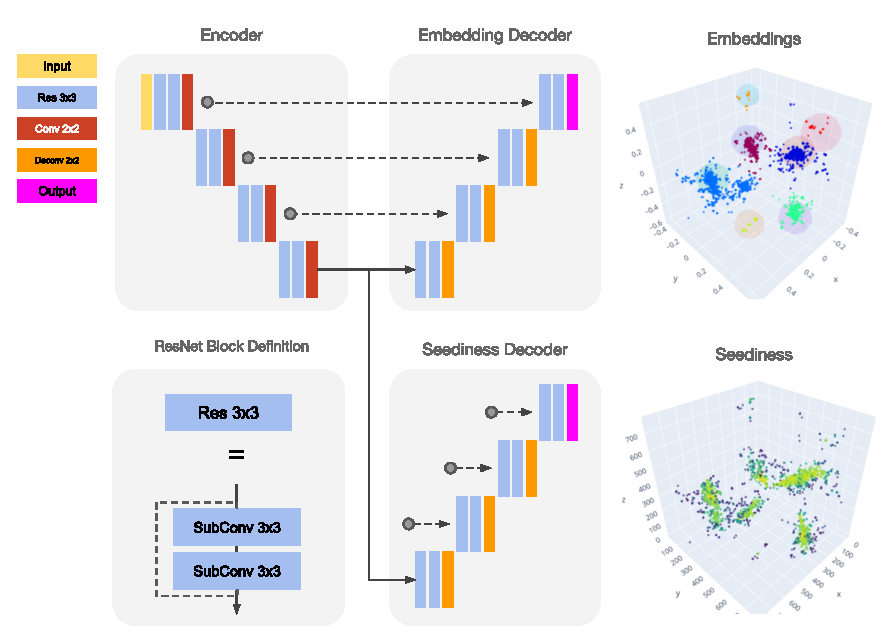
\includegraphics[width=0.98\textwidth]{figures/spice_architecture.pdf}
    \caption{Comparison of true underlying clusters (left) and the reconstructed clusters (right) by SPICE. Discrete colors are assigned to the pixels that belong to the same cluster.  }
    \label{fig:clustering:spice_architecture}
\end{figure*}
\begin{figure*}[t]
    \centering
    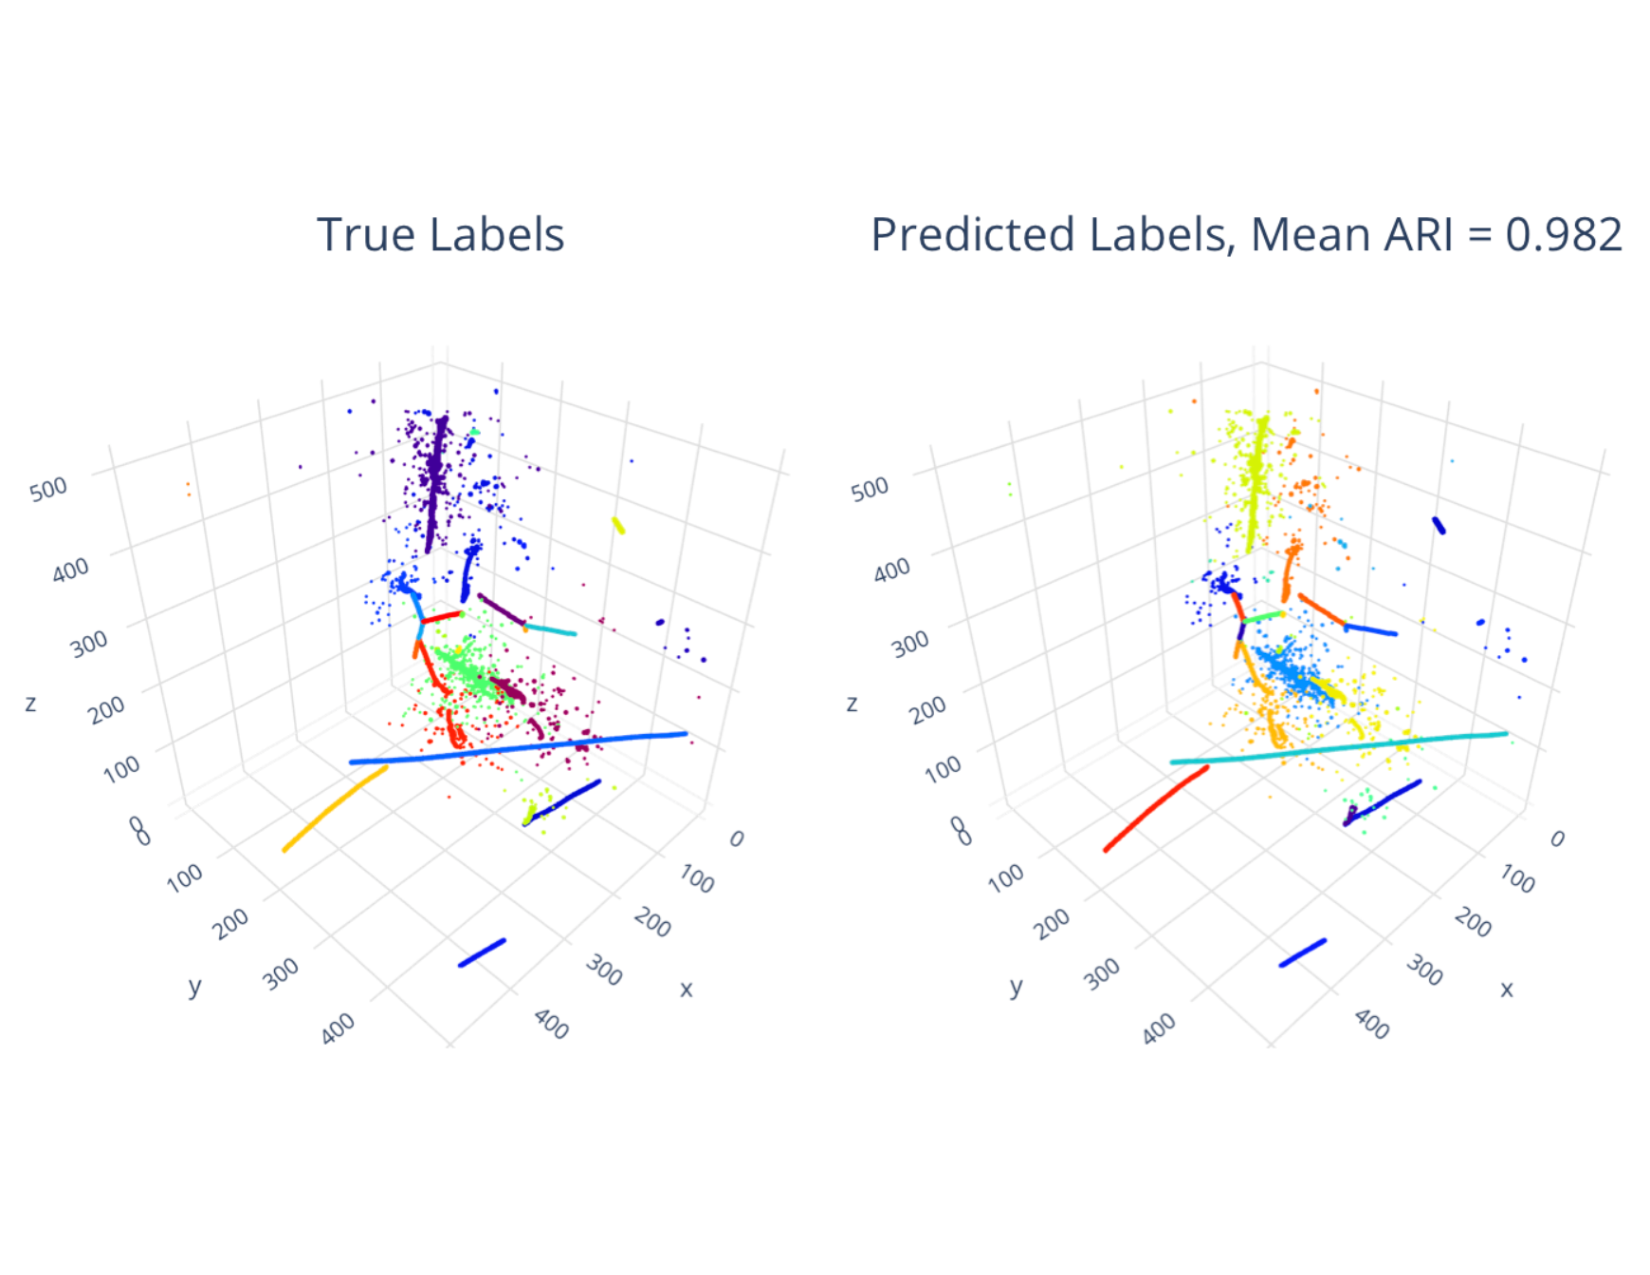
\includegraphics[width=0.98\textwidth,trim=0cm 3cm 0cm 3cm, clip]{figures/prediction_5.pdf}
    \caption{Comparison of true underlying clusters (left) and the reconstructed clusters (right) by SPICE. Discrete colors are assigned to the pixels that belong to the same cluster.  }
    \label{fig:clustering:spice_clustering}
\end{figure*}

SPICE combines this  preceding research~\cite{disc,8953222} with the U-ResNet architecture as a backbone as shown in Figure~\ref{fig:clustering:spice_architecture}. The decoder is split into two branches where one branch is responsible learning a transformation function into the embedding space and the margin value and the other branch estimates the seediness score. An example output from their study~\cite{koh2020scalable} is shown in Figure~\ref{fig:clustering:spice_clustering}. The adjusted Rand index~\cite{ari}, a standard metric for pixel clustering in image analysis, is above 0.98 for this image, which indicates nearly perfect clustering. SPICE is the first purely 3D pixel clustering algorithm proposed for LArTPC experiments where the interaction vertex is unknown and can be anywhere in the detector. It is expected to be used for analyzing 3D image data from the DUNE near detector, a pixel-based 3D imaging LArTPC.

Despite the successful introduction of SPICE, which is meant to overcome a challenge of object occlusions faced by proposal-based approach, it should be noted that SPICE is subject to its own limitations because it uses CNNs. For example, consider a muon with a very long trajectory. For an algorithm like SPICE to transfer all pixels from image space to the centroid of a cluster in embedding space, {\it somehow} pixels need to communicate a common target location. Yet, how far such information can reach between distant pixels, called the size of {\it receptive field}, depends on the CNN architecture as it requires convolution or down-sampling operations. The limitation ultimately comes from the fact that CNN kernels only connect, or combine features from, neighbor pixels. This could be overcome by using GNNs, in which edges can be defined between distant nodes to enable distant information passing without extra operations, while keeping the same objectives and loss definitions employed by SPICE. We shall focus on {\it particle clustering} in the next section. The advantage becomes more apparent and the choice of GNN as an underlying architecture is more natural.

\section{Clustering Particles Using Graph Neural Networks}
Clustering in particle physics data reconstruction is naturally a hierarchical task. Among the examples covered in this chapter, pixels  may be clustered into individual particle trajectory, then some particles may be clustered into single interaction as the shared origin. An intermediate particle representation may be also useful, such as an electromagnetic shower which consists of many trajectories of individual electrons and positrons, or a neutral pion represented by two decay gamma rays. While CNNs provide a natural representation for a matrix-formatted image data, generalization is needed for a higher level data representations such as clusters. A graph representation, in which constituents and their correlations are represented as nodes and edges respectively, provides a generalized input and output data representating a clustering task at different levels. 

With GNNs, a clustering task can be solved in the form of a binary edge classifications. Simply put, those nodes connected by {\it valid} edges belong to the same cluster, and disconnected nodes, or the nodes connected by {\it invalid} edges, do not.  While this sounds simple, implementations vary wildly due to the flexibility in designing the GNNs. Important considerations include the initial graph construction, operations to extract node and edge features from input data, static v.s. dynamic graph (i.e. a dynamic graph may generate/erase new/existing nodes/edges), operations for updating node and edge features, {\it message passing}, a mechanism to propagate information throughout the graph, and lastly a post-processing or interpretation of the graph nodes and edges in the final state. This manuscript focus on a comprehensive study of GNN architectures for LArTPC particle and interaction clustering applications described below~\cite{drielsma2020clustering}. Other notable examples include clustering of hits for tracking and calorimeters in the ATLAS and the CMS experiments respectively~\cite{ju2020graph}, and they are covered by other authors in the GNN chapter.

%\subsection{Partitioning Many Particle Pile-ups at LHC}
%One of the first application of GNNs in the Large Hadron Collider~\cite{Evans_2008} (LHC) experiments including ATLAS~\cite{Collaboration_2008} and CMS~\cite{Chatrchyan:2008aa} is a track reconstruction, which is to identify the right combination of detector hits to form a particle trajectory. A serious challenge will arise at the High Luminosity LHC (HL-LHC) in the future where a pile-up of $\mathcal{O}(10^4)$ tracks are expected with $\mathcal{O}(10^5)$ detector hits. All of these tracks, sparsely sampled with 10~hits per track on average, originate from the interaction vertex and travel radially outward. Hits are recorded by the layers of a cylindrical detectors, and a track is formed by connecting hits across sylindrical layers. It is essentially a combinatorial search to find the right partition, or cluster, of hits. As the existing algorithm is not considered scalable to the level of HL-LHC, a GNN is proposed as a new solution and has shown promising performance~\cite{ju2020graph}.

%The layout of the detector consists of multiple cylindrical barrels where hits are detected. The initial graph is constructed with a hit position in the cylindrical coordinate, $(r,\phi,z)$ and edges that connect hits between adjacent detector layers with a diff vector between two nodes as edge features. There are two MLPs with two hidden layers each for encoding the input edge and node features to the latent feature array $H_0$, and other two MLPs with two hidden layers for updating the node and edge features respectively. $H_0$ is concatenated to a derived latent feature array after every iteration of updating the graph. The last layer performs a sigmoid operation to produce a normalized score value ranging from 0 to 1. This seemingly minimal, yet fast and scalable architecture, can identify 95.9~\% of edges correctly with a threshold value of 0.5 on the edge score, which translates into 95~\% of accurately reconstructed tracks~\cite{ju2020graph}. 

%A similarly simple GNN shows a promising performance on clustering the hits in the CMS High-Granularity Calorimeter by the same research team~\cite{ju2020graph}. In case of a calorimeter, a node can have heterogeneous edges with neighboring nodes unlike a track reconstruction, and an update of node features is done by aggregating features from all connected edges, referred to as ``EdgeConv'' by DGCNN authors. The initial graph is constructed with hits and edges that connect k-Nearest-Neighbors (kNNs). Unlike the GNN for tracking, the initial features $H_0$ is not aggregated to each node update, and instead all intermediate features $H_i$ after $i$-th update are aggregated to an input to the final layer. The performance study is done using simulation of single particles for a muon, a pion, and a photon. An efficiency and a purity are found to be 99~\% and 90~\% for muons respectively. For photons, both efficiency purity are 99~\%. For pions, both efficiency and purity are more than 90~\%. While having a promising performance, this GNN architecture is small, fast, and thus scalable to a larger, more complex calorimetry data samples.



\subsection{Clustering Electromagnetic Shower Fragments}
\begin{figure*}[t]
    \centering
    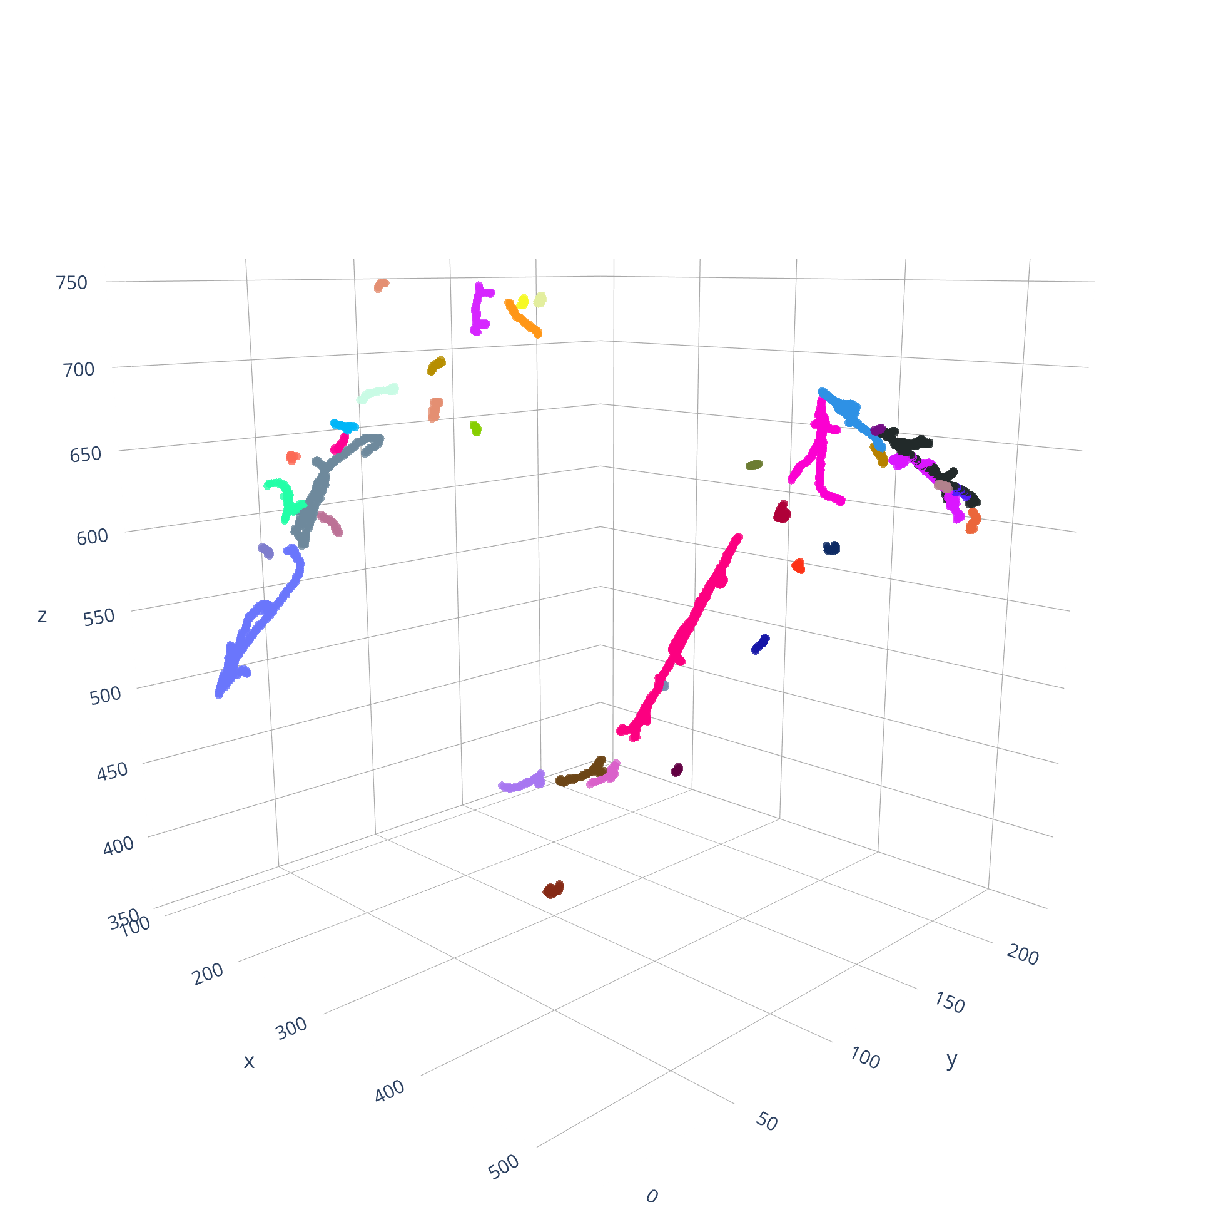
\includegraphics[width=0.98\textwidth]{figures/fragments.pdf}
    \caption{Shower fragments produced by running DBSCAN on shower pixels. The color scale is discrete and pixels that belong to the same fragment cluster share the same color.}
    \label{fig:clustering:gnn_input}
\end{figure*}
An electromagnetic shower may contain many small fragments of electron and positron trajectories that need to be clustered together. The radiation length is large (15--30~cm) as compared to $\approx$mm per pixel image resolution, which causes a gap between fragments of varying size, from a few to hundreds of pixels. Following the success of highly accurate semantic segmentation techniques~\cite{domine_laura_2018_1300713}, a GNN solution~\cite{drielsma2020clustering} is proposed and demonstrated  promising performance. First, DBSCAN is run only on the shower pixels identified by U-ResNet, a semantic segmentation model. This produces many small fragments of electromagnetic showers as shown in Figure~\ref{fig:clustering:gnn_input}, taken from the original paper. A graph is constructed by taking each fragment as a node and a connection between fragments as an edge. 

\begin{figure*}[t]
    \centering
    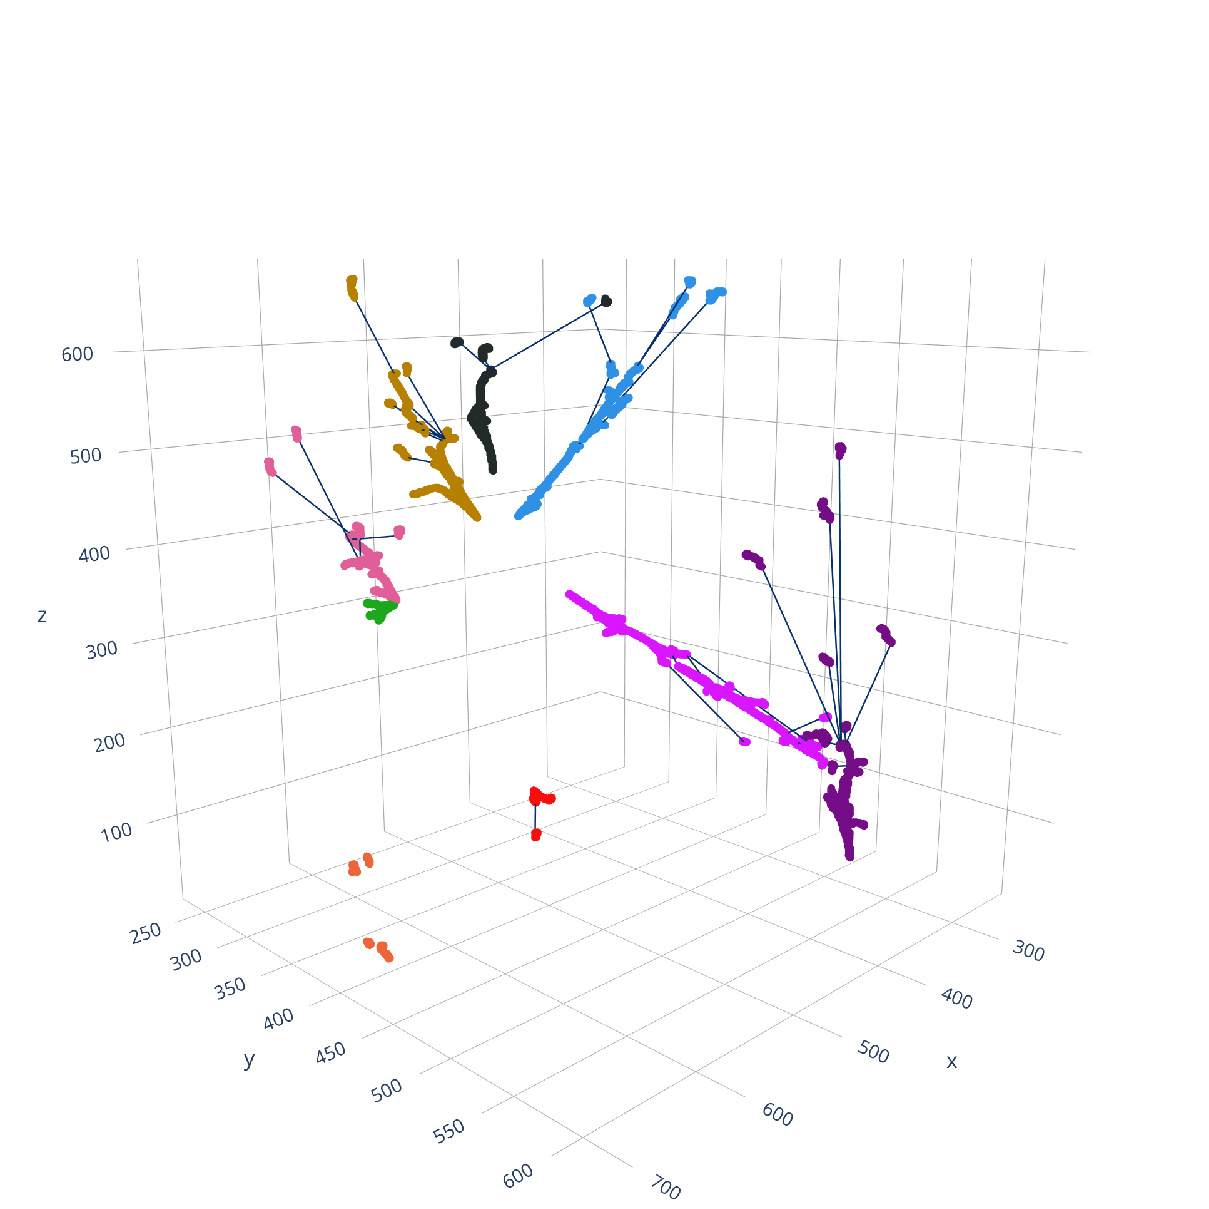
\includegraphics[width=0.495\textwidth,trim=1cm 0cm 1cm 3cm, clip]{figures/event_11512_label.pdf}
    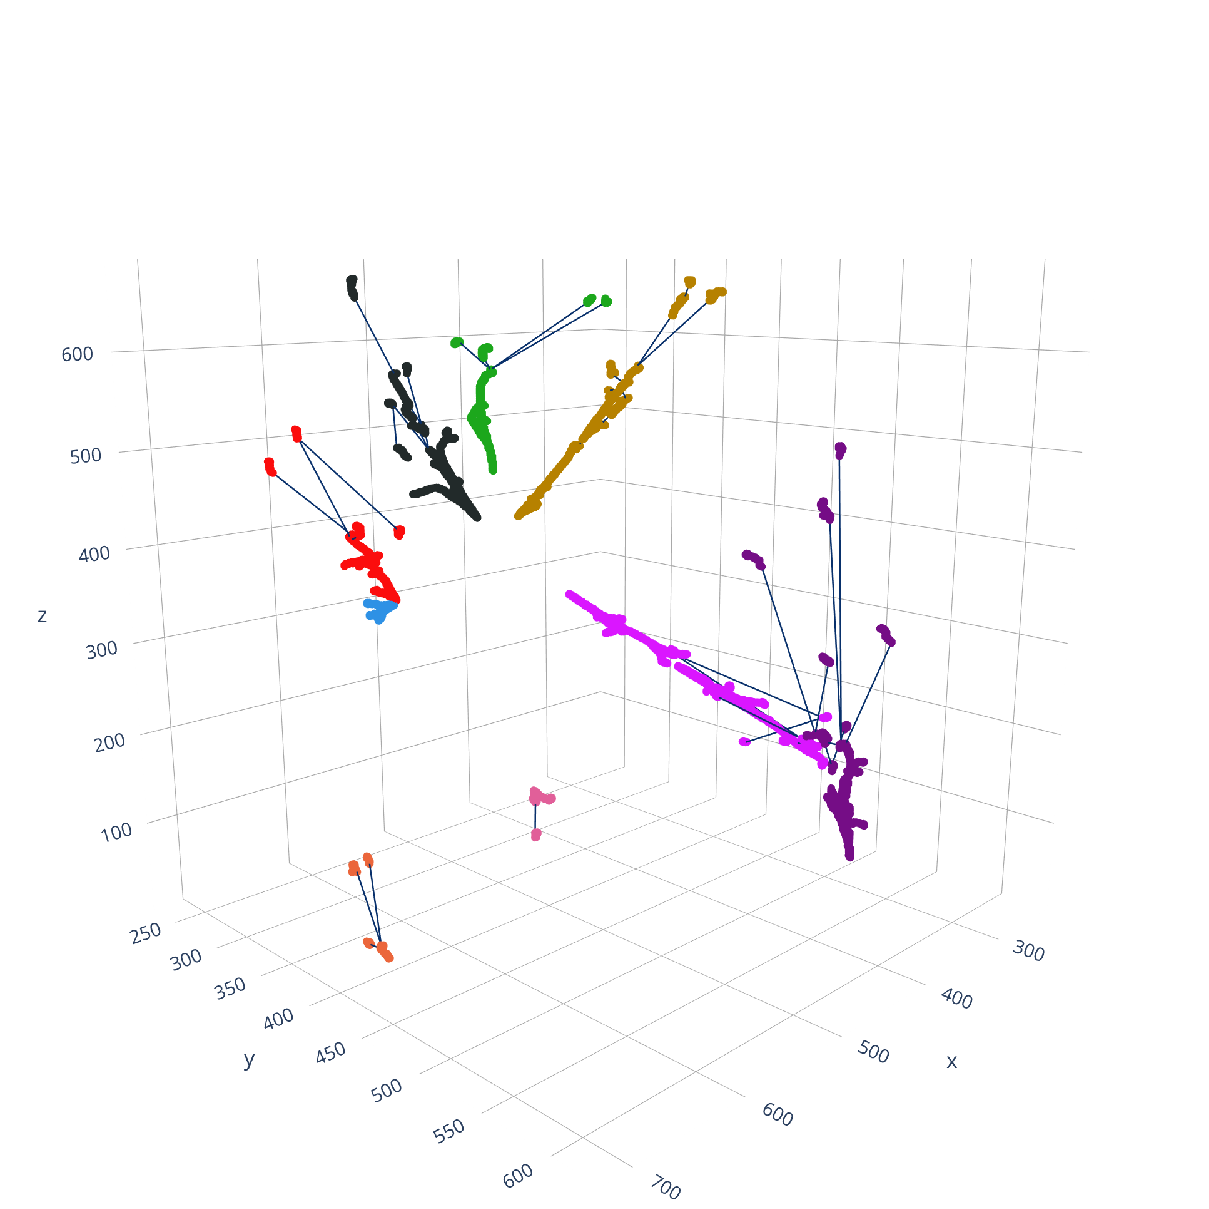
\includegraphics[width=0.495\textwidth,trim=1cm 0cm 1cm 3cm, clip]{figures/event_11512_pred.pdf}
    \caption{Left: the true underlying clusters (color) of electromagnetic shower fragments with true edges defined based on the flow of particles. Right: the inferred clusters and edges using GNN. }
    \label{fig:clustering:gnn_output}
\end{figure*}
In addition to the edge classification, a GNN in this study is trained jointly for a node classification in order to identify a {\it primary} node, or the root fragment of the shower. This is important as the primary fragment is most informative in terms of the start position and the initial direction of the shower. The authors of this work explored a variety of options at all stages of the problem solving including:
\begin{itemize}
    \item input graph construction methods including a complete graph, edges in Delaunay triangulation, minimum spanning tree (MST), and 5 nearest neighbors,
    \item encoding methods for the initial node and edge features including geometrical features, addition of shower start position from PPN, a sparse CNN encoder as a learnable feature extractor from the pixel level,
    \item message passing mechanisms including \verb|MetaLayer|~\cite{inductive_bias}, \verb|NNConv|~\cite{nnconv}, \verb|EdgeConv|~\cite{edgeconv}, \verb|GATConv|~\cite{gatconv}, and \verb|AGNNConv|~\cite{agnnconv},
    \item the repetition count of a message passing operation,
    \item two target graph definitions including a cluster graph, a disjoint union of a complete graph, and a ``forest'', a collection of trees where each tree represent a particle flow within each shower.
\end{itemize}
Skipping the discussion details, which can be found in their paper, the recommended choice for this clustering task is a complete graph as an input, geometrical features with the shower start position from PPN to define the initial node and edge features, \verb|MetaLayer| for message passing, three rounds of message passing, and a cluster graph as an optimization target. Figure~\ref{fig:clustering:gnn_output} shows an example inference output under this configuration. Overall, the reported clustering purity and efficiency are both 99.5~\%, and achieves 97.7~\% for the adjusted Rand index~\cite{ari} (ARI) clustering performance metric. The node classification accuracy, which is to identify the primary fragment of a shower, is reported as 99.77~\%.

\subsection{Clustering Loss by a Classification of Graph Edges} 
\begin{figure*}[t]
    \centering
    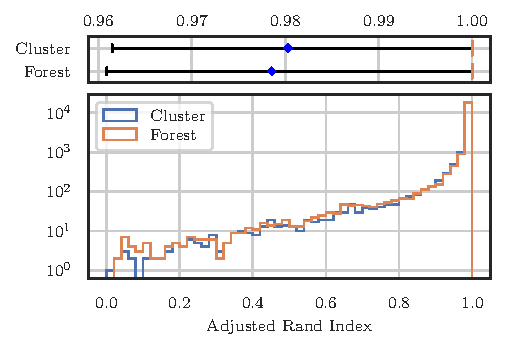
\includegraphics[width=0.75\textwidth]{figures/target_edge_pred_clustering_metrics.pdf}
    \caption{Comparison of different target graphs, a cluster graph v.s. a forest, using the ARI metric for clustering of electromagnetic showers.}
    \label{fig:clustering:gnn_diff_target}
\end{figure*}
Two observations in the study of electromagnetic shower clustering~\cite{drielsma2020clustering} are worth noting. The first is a comparison of two target cluster types: a cluster graph and a forest. A derivation of the latter is a more challenging task as the edges in a correct tree are a subset of edges in a cluster graph, hence requiring more discrimination power. In turn, a forest prediction provides not only a cluster, but also a particle flow within a shower. As a pleasant surprise, the final clustering performance between two target graphs are nearly identical as shown in Figure~\ref{fig:clustering:gnn_diff_target}. This seems promising to extend the same approach for a generic particle flow reconstruction using a GNN with directed edge.

The second point is an obvious, yet an important remark that is often missed. Quoting exactly from the paper, {\it ``The network predicts an edge score matrix, $\bm{S}^e$, which tries to replicate the predefined ground-truth adjacency matrix, $\bm{A}$. In a graph partition problem, $\bm{A}$ should be designed such that, if $a_{ij}=1$, then nodes $i$ and $j$ belong to the same group. The converse statement does not have to hold, as nodes $i$ and $j$ may not be connected directly as long as they are linked through an indirect path.''} In other words, running an inference simply by turning on/off graph edges based on individual score may not result in the most optimal graph, or equivalently, that may result in a larger loss. In the paper, the authors give a further clarification using two cluster graphs connected by two edges with score values 0.1 and 0.6. If one naively interpret the edge with a score 0.6 as a valid edge, this results in merging two clusters, which is equivalent to enable the other edge of a lower score value of 0.1. As a result, the overall loss may become larger than two disjoint cluster graphs. Without this consideration, the approach using a cluster target is much more prone to incorrectly merging two clusters due to any edge between them with a score value above 0.5. 


\subsection{Clustering Interactions} 
\begin{figure*}[t]
    \centering
    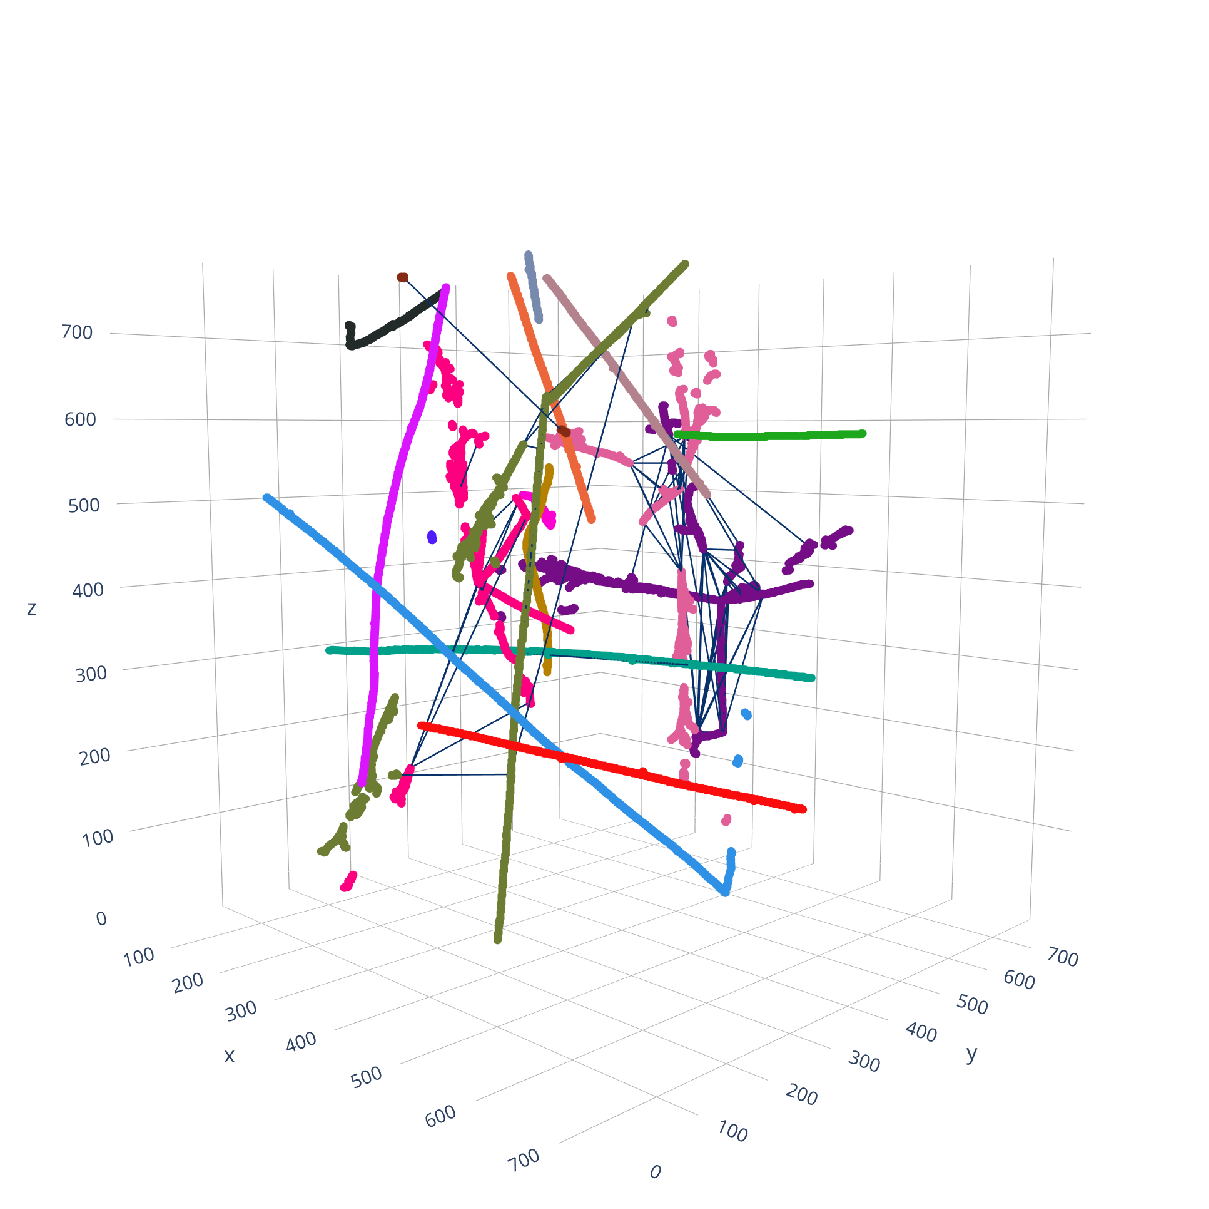
\includegraphics[width=0.495\textwidth,trim=1cm 0cm 1cm 3cm, clip]{figures/event_2138_4985_18647_20468_label.pdf}
    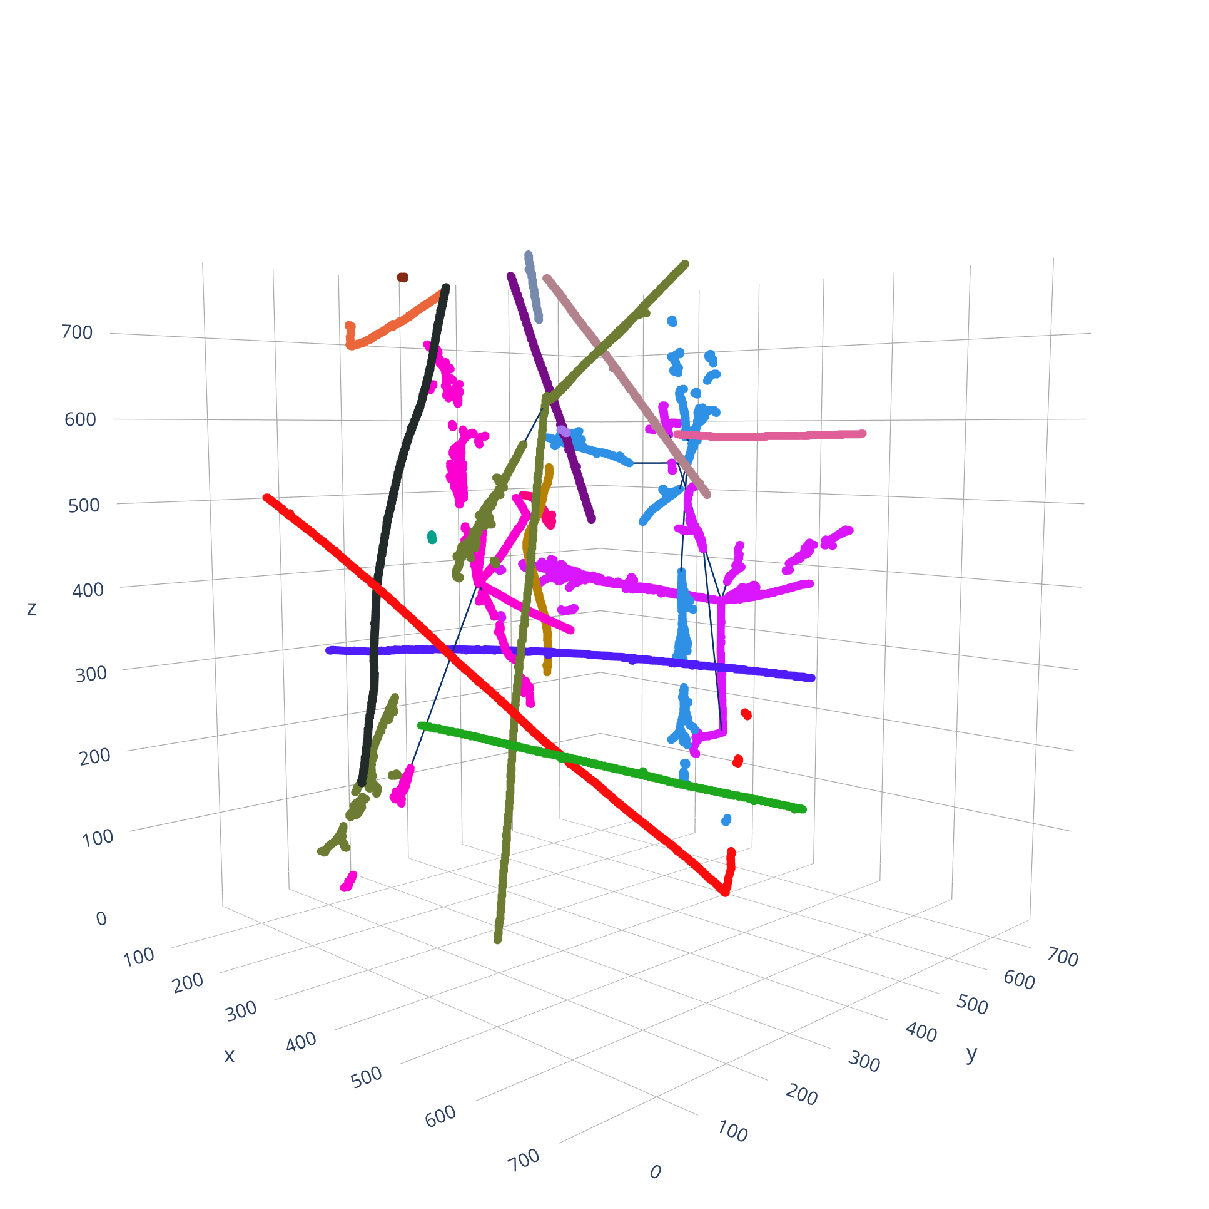
\includegraphics[width=0.495\textwidth,trim=1cm 0cm 1cm 3cm, clip]{figures/event_2138_4985_18647_20468_pred.pdf}
    \caption{Left: the true underlying clusters (color) of particles with true edges defined based on the particle flow. Right: the inferred clusters and edges using GNN. The ARI for this randomly selected event is 100~\% (perfect).}
    \label{fig:clustering:gnn_output_interaction}
\end{figure*}
GNN can provide a generalized clustering framework as noted above, and this is demonstrated by applying the same architecture at the next stage of a reconstruction chain, clustering of particles into a group that shares the same origin interaction. At this stage, a graph node is a particle of any type, including both track and shower particles. A graph pooling operation may be used to aggregate features from clustered fragments for shower particles. This is, however, not done in the paper, and instead the node and edge features are derived using similar methods employed at the shower clustering stage, namely geometrical features computed from analytical functions, PPN output, and a particle's semantic type from U-ResNet. An example output image is shown in Figure~\ref{fig:clustering:gnn_output_interaction}. 

Due to a high intensity neutrino beam for the DUNE program, the DUNE near detector (DUNE-ND), a 3D imaging LArTPC, is expected to observe a ``pile-up'' of more than 20 neutrino interactions per image for the first time in the history of experimental neutrino physics. It is one of the hardest data reconstruction challenges yet to be addressed. The GNN-based particle clustering technique shows a strong promise to address this challenge. In the paper~\cite{drielsma2020clustering}, the mean values of a purity, efficiency, and ARI of particle clustering are all above 99~\% for images in  which particle density per unit volume is comparable to DUNE-ND. 

%\section{Closing}
%Clustering methods are the core part of data reconstruction software in particle physics, and also it is a high traffic cross-road with ML research in computer vision as well as an area of geometric and topological learning.  While traditional ML techniques have been utilized for clustering tasks for a long time, modern ML algorithms remain to be explored in more depth. A high flexibility of GNN architectures may be exploited to introduce more inductive bias, and a causal structure may be introduced using a dynamic tree/forest graph models with directional edges. Backed with a strong history of success and its natural fit for analyzing particle imaging detector data in neutrino physics, (sparse) CNNs are expected to continue playing an important role as well.  


\bibliographystyle{ws-rv-van}
\bibliography{references}

%\blankpage
%\printindex[aindx]                 % to print author index
%\printindex                         % to print subject index

\end{document}
